%% Basierend auf einer TeXnicCenter-Vorlage von Mark M�ller
%%%%%%%%%%%%%%%%%%%%%%%%%%%%%%%%%%%%%%%%%%%%%%%%%%%%%%%%%%%%%%%%%%%%%%%

% W�hlen Sie die Optionen aus, indem Sie % vor der Option entfernen  
% Dokumentation des KOMA-Script-Packets: scrguide

%%%%%%%%%%%%%%%%%%%%%%%%%%%%%%%%%%%%%%%%%%%%%%%%%%%%%%%%%%%%%%%%%%%%%%%
%% Optionen zum Layout des Buchs                                     %%
%%%%%%%%%%%%%%%%%%%%%%%%%%%%%%%%%%%%%%%%%%%%%%%%%%%%%%%%%%%%%%%%%%%%%%%
\documentclass[a4paper, 11pt,
	%a5paper,							% alle weiteren Papierformat einstellbar
	%landscape,						% Querformat
	%10pt,								% Schriftgr��e (12pt, 11pt (Standard))
	%BCOR1cm,							% Bindekorrektur, bspw. 1 cm
	%DIVcalc,							% f�hrt die Satzspiegelberechnung neu aus
	%											  s. scrguide 2.4
	%oneside,							% einseitiges Layout
	%twocolumn,						% zweispaltiger Satz
	openany,							% Kapitel k�nnen auch auf linken Seiten beginnen
	%halfparskip*,				% Absatzformatierung s. scrguide 3.1
	headsepline,					% Trennline zum Seitenkopf	
	footsepline,					% Trennline zum Seitenfu�
	%notitlepage,					% in-page-Titel, keine eigene Titelseite
	%chapterprefix,				% vor Kapitel�berschrift wird "Kapitel Nummer" gesetzt
	%appendixprefix,				% Anhang wird "Anhang" vor die �berschrift gesetzt
	%normalheadings,			% �berschriften etwas kleiner (smallheadings)
	%idxtotoc,						% Index im Inhaltsverzeichnis
	%liststotoc,					% Abb.- und Tab.verzeichnis im Inhalt
	%bibtotoc,						% Literaturverzeichnis im Inhalt
	%leqno,								% Nummerierung von Gleichungen links
	%fleqn,								% Ausgabe von Gleichungen linksb�ndig
	%draft								% �berlangen Zeilen in Ausgabe gekennzeichnet
	bibliography = totoc,			% include bib in toc
	listof=totoc,				% include listof entries in toc
	listof=entryprefix,				% include listof entries in toc
	titlepage= on,				% own page for each title page
	captions= tableabove, %platzierung der Beschreibung
	%tocindent,
	ngerman
	%,bibtotocnumbered
]
{scrbook}
%% Bibliographiestil %%%%%%%%%%%%%%%%%%%%%%%%%%%%%%%%%%%%%%%%%%%%%%%%%%
%\usepackage{natbib}
\usepackage[
	backend     = biber,
	natbib      = true,
	style       = alphabetic,
	sorting     = nyt,
	date     		= long,
	urldate     = long,
	maxbibnames = 99
]{biblatex}
\addbibresource{Literatur.bib}
\DeclareNameAlias{sortname}{last-first}
\usepackage[babel,german=quotes]{csquotes}

%\pagestyle{empty}		% keine Kopf und Fu�zeile (k. Seitenzahl)
%\pagestyle{headings}	% lebender Kolumnentitel  
%\setuptoc{toc}{numbered}

%% Deutsche Anpassungen %%%%%%%%%%%%%%%%%%%%%%%%%%%%%%%%%%%%%
\usepackage[latin1]{inputenc} %  Alternativ unter Windows
\usepackage[T1]{fontenc}
\usepackage[ngerman]{babel}
\usepackage{mathptmx} % Hier steckt Times drin

\usepackage{lmodern}

\usepackage[margin = 10pt, labelfont=bf]{caption}						% table headers


\usepackage{hyperref}
\usepackage[normalem]{ulem}
\usepackage{url}
%% Falls die automatische Worttrennung in W�rtern mit Umlauten
%% nicht funktionieren sollte oder der Text pixelig aussieht:
%% ==> Installieren Sie die cm-super Fonts (z.B. mit dem mikTeX Package Manager).
%% Eine nicht ganz vollwertige Alternative ist die Verwendung dieses Pakets:
%\usepackage{ae, aeguill}

\usepackage{listings}								%Quellcode
%% tables
\usepackage{multicol} 							% multiple columns in tables
\usepackage{multirow}								% multiple rows in tables
\usepackage{hhline}									% horizontal lines
\usepackage{longtable}							% pagebreak tables
\usepackage{booktabs}								% bold table lines, e.g. \toprule
\usepackage{tabularx}								% neue Tabular-Umgebung

% Tabellen Farbe
\usepackage{colortbl}
\usepackage{xcolor}

%% Packages f�r Grafiken & Abbildungen %%%%%%%%%%%%%%%%%%%%%%
\usepackage{graphicx} %%Zum Laden von Grafiken
\usepackage{float} % unterdr�ckt, dass Bilder ins falsche Kapitel getan werden (mit eckiger Klammer mit [H])

%\usepackage{subfig} %%Teilabbildungen in einer Abbildung
%\usepackage{pst-all} %%PSTricks - nicht verwendbar mit pdfLaTeX

%% Beachten Sie:
%% Die Einbindung einer Grafik erfolgt mit \includegraphics{Dateiname}
%% bzw. �ber den Dialog im Einf�gen-Men�.
%% 
%% Im Modus "LaTeX => PDF" k�nnen Sie u.a. folgende Grafikformate verwenden:
%%   .jpg  .png  .pdf  .mps
%% 
%% In den Modi "LaTeX => DVI", "LaTeX => PS" und "LaTeX => PS => PDF"
%% k�nnen Sie u.a. folgende Grafikformate verwenden:
%%   .eps  .ps  .bmp  .pict  .pntg
\usepackage{latexsym}
\usepackage{amsmath, amssymb, amsthm}
\usepackage{geometry}
%\usepackage{tocloft}

\usepackage{scrpage2}
\pagestyle{scrheadings}
%% \usepackage[authoryear]{natbib}
%% \bibliographystyle{alpha}


\definecolor{light-gray}{gray}{0.95}
%%%%%%%%%%%%%%%%%%%%%%%%%%%%%%%%%%%%%%%%%%%%%%%%%%%%%%%%%%%%%%%%%%%%%%%%%%%%%%%
%%Seitenlayout definieren
\geometry{a4paper,
  left  = 25mm,
  right = 20mm,
  top   = 2.5cm,
  bottom= 3cm,
}

%%%%%%%%%%%%%%%%%%%%%%%%%%%%%%%%%%%%%%%%%%%%%%%%%%%%%%%%%%%%%%%%%%%%%%%%%%%%%%%
%% Quellenformatierung für Tabellen und Grafiken
\newcommand*{\quelle}[1]{%
	\footnotesize(\uline{Quelle:} #1)
}

%%%%%%%%%%%%%%%%%%%%%%%%%%%%%%%%%%%%%%%%%%%%%%%%%%%%%%%%%%%%%%%%%%%%%%%%%%%%%%%
%% Quellenformatierung für Tabellen und Grafiken
\newcommand*{\tableRowHeader}[1]{%
	\cellcolor{lightgray}\textbf{\underline{#1}}
}
%%%%%%%%%%%%%%%%%%%%%%%%%%%%%%%%%%%%%%%%%%%%%%%%%%%%%%%%%%%%%%%%%%%%%%%%%%%%%%%
%% Fuß- und Kopfzeile bei Kapitelseiten:
\renewcommand{\chapterpagestyle}{scrheadings}

%%%%%%%%%%%%%%%%%%%%%%%%%%%%%%%%%%%%%%%%%%%%%%%%%%%%%%%%%%%%%%%%%%%%%%%%%%%%%%%
%% Untersteichen der Chapter und subchapter
%\RedeclareSectionCommands[font=\normalsize]{chapter,section,subsection,subsubsection}

\renewcommand*{\chapterlinesformat}[3]{%
  #2\uline{#3}%
}
\renewcommand*{\sectionlinesformat}[4]{%
  \hskip#2#3\uline{#4}% 
}

%%%%%%%%%%%%%%%%%%%%%%%%%%%%%%%%%%%%%%%%%%%%%%%%%%%%%%%%%%%%%%%%%%%%%%%%%%%%%%%
%%% Tabellen und Abbildungs Verzeichniss formatierung: Es iwrd so formatier, dass
%%% Prfäx Fettgedruckt und getrent zum Text mit einem : ist (Quelle: https://komascript.de/node/1911)
\addtokomafont{captionlabel}{\bfseries} %nötig, für fettdruck
\addtokomafont{captionlabel}{\uline} %nötig, für unterstrich

%Grafik
\renewcommand*\listoflofentryname{\bfseries\figurename}
	%\renewcaptionname{ngerman}{\figurename}{Abb.}
\BeforeStartingTOC[lof]{\renewcommand*\autodot{:}}

%Tabellen
\renewcommand*\listoflotentryname{\bfseries\tablename}
\BeforeStartingTOC[lot]{\renewcommand*\autodot{:}}

%%%%%%%%%%%%%%%%%%%%%%%%%%%%%%%%%%%%%%%%%%%%%%%%%%%%%%%%%%%%%%%%%%%%%%%%%%%%%%%
%%%% Im Text Tab. und Abb. Captions werden Fett und unterstrichenn ausgegeben
\makeatletter
\renewcommand\caption@@make[2]{%
  \centering\underline{\textbf{#1:}}~#2}
\makeatother
%%%%%%%%%%%%%%%%%%%%%%%%%%%%%%%%%%%%%%%%%%%%%%%%%%%%%%%%%%%%%%%%%%%%%%%%%%%%%%%
%%%Tabellenformatierung
%Tabellenverzeichnis
\lstset{
    frame = LL, 										% draw a frame at the top and bottom of the code block
    tabsize = 4, 									% tab space width
    showstringspaces = false, 	% don't mark spaces in strings
    numbers=left, 							% display line numbers on the left
    commentstyle=\color{green}, % comment color
    keywordstyle=\color{blue}, 	% keyword color
    stringstyle=\color{red} 		% string color
}
\lstdefinelanguage{json}{
    string=[s]{"}{"},
    stringstyle=\color{blue},
    comment=[l]{:},
    commentstyle=\color{black},
}



\pagestyle{scrheadings}
\automark[chapter]{chapter}


\begin{document}

\pagestyle{scrheadings}
\clearscrheadfoot
\ihead{\headmark}
\ofoot{Seite  $\vert$ \pagemark}
%%%%%%%%%%%%%%%%%%%%%%%%%%%%%%%%%%%%%%%%%%%%%%%%%%%%%%%%%%%%%%%%%%%%%%%
%% Ihr Buch                                                          %%
%%%%%%%%%%%%%%%%%%%%%%%%%%%%%%%%%%%%%%%%%%%%%%%%%%%%%%%%%%%%%%%%%%%%%%%
%% Schmutztitel-Seite %%%%%%%%%%%%%%%%%%%%%%%%%%%%%%%%%%%%%%%%%%%%%%%%%
%\extratitle{Schmutztitel}

%% eigene Titelseitengestaltung %%%%%%%%%%%%%%%%%%%%%%%%%%%%%%%%%%%%%%%
% Titelblatt der Arbeit
\thispagestyle{empty}

% Header
\begin{titlepage}
\fontsize{12pt}{13pt}\selectfont

	\begin{minipage}{0.18\textwidth}
		
\includegraphics[width=1\textwidth]{logo/Beuth-Logo_single}
	\end{minipage}
	\begin{minipage}{1\textwidth}
			Beuth Hochschule f�r Technik\\
			Fachbereich VI - Informatik und Medien\\
			Luxemburger Stra�e 10\\
			13353 Berlin
	\end{minipage}
	
	\begin{center}

	\vspace*{2.5cm} {\textbf{ \large MASTERARBEIT}
	\\zur Erlangung des akademischen Grades\\ \textbf{Master of Science}\\
	\vspace*{0.50cm} {im Rahmen des Studiums\\\\ \textbf{Medieninformatik}\\}
	\vspace*{1.5cm} {\textbf{\Large Entwicklung einer Softwarel�sung zum Energiemonitoring}}
	\vspace*{1.5cm} \\ {vorgelegt von\\}
	\vspace{0.5cm} {\large \textbf{Dogan A,}\\Matrikelnummer: s123456\\}
	\vspace{0.5cm} {\large E-Mail: do.al@gmx.net\\}
	\vspace{1.5cm} {\large Berlin, den \today}



%\vspace{4.5cm}

\vspace*{\fill}
\vspace*{1.5cm}
\begin{table}[h]
	\begin{tabular}{ll}
		%Aufgabensteller & Prof. \\ 
		%Durchgef�hrt bei: & Firmenname\\ 
		%Betreuer: & Betreuer Firma\\ 
		Betreuer:  & Prof Dr. Joachim \\
		Gutachter: & Prof Dr. Alfred
	\end{tabular}
\end{table}

 \end{center}

\fontsize{11}{11}
\end{titlepage}
\pagenumbering{Roman}
\setcounter{page}{1}

%% Angaben zur Standardformatierung des Titels %%%%%%%%%%%%%%%%%%%%%%%%
%\titlehead{Titelkopf}
%\subject{Typisierung}
%\title{}
%\author{Ihr Name}
%\and{Der Name des Co-Autoren}
%\thanks{Fu�note}			% entspr. \footnote im Flie�text
%\date{}							% falls anderes, als das aktuelle gew�nscht
%\publishers{Herausgeber}

%% R�ckseite der Titelseite %%%%%%%%%%%%%%%%%%%%%%%%%%%%%%%%%%%%%%%%%%%
%\uppertitleback{Titelr�ckseitenkopf}
%\lowertitleback{Titelr�ckseitenfu�}

%% Widmungsseite %%%%%%%%%%%%%%%%%%%%%%%%%%%%%%%%%%%%%%%%%%%%%%%%%%%%%%
%\dedication{Widmung}

%\maketitle 						% Titelei wird erzeugt

%% Erzeugung von Verzeichnissen %%%%%%%%%%%%%%%%%%%%%%%%%%%%%%%%%%%%%%%
\tableofcontents			% Inhaltsverzeichnis
%\listoftables				% Tabellenverzeichnis
%\listoffigures				% Abbildungsverzeichnis



%% Der Text %%%%%%%%%%%%%%%%%%%%%%%%%%%%%%%%%%%%%%%%%%%%%%%%%%%%%%%%%%%
\mainmatter					% Vorspann (z.B. r�mische Seitenzahlen)

\pagenumbering{arabic}

\chapter{Einleitung}
\label{sec:KapEinleitung}
Energie ist f�r vieles n�tig. Ohne Energie w�ren die bisherige industrielle Entwicklung
und das Leben wie es bekannt ist, nicht m�glich. Erst Energietr�ger wie �l, Erdgas und
vor allem elektrische Energie sollen den wirtschaftlichen und technischen Fortschritt
erst erm�glichen haben \cite[vgl.][S. 4 - S. 6]{Bpb2013} and \cite[vgl.][S. 4 - S. 6]{Bpb2013}. 2014 wurden 684 TWh Strom
erzeugt. Die Quelle der erzeugten elektrischen Energien wurden vor allem durch
fossile Brennstoffe erzeugt \cite[vgl.][S.38]{EDG}.

Aufgrund des Energieverbrauchs finden auch Klima�nderungen durch Umweltverschmutzung,
verursacht durch Treibhausgase wie Kohlendioxid, statt. Dies hat nicht nur eine
steigende globale Durchschnittstemperatur, sondern auch extreme Wetterereignisse,
wie St�rme und �berflutungen zur Folge \cite[vgl.][]{Ven2013}. Die globale Durchschnittstemperatur
soll um bis zu vier Grad Celsius steigen, wenn nichts dagegen unternommen wird.

Die Reduzierung des Stromverbrauchs hat nicht nur klimasch�tzende, sondern auch
Kosten reduzierende Wirkung, da verminderte Nachfrage und Verbrauch auch entsprechend
niedrigere Ausgaben f�r Strom bedeuten. Die Kontrolle des eigenen Energieverbrauchs
wird daher immer wichtiger. Damit ist nicht nur die �berwachung der eigenen Energiekosten
m�glich, sondern auch die Steigerung der Energieeffizienz von Anlagen \cite[vgl.][]{pae}.
Zudem wird durch die Energieverbrauchskontrolle die M�glichkeit er�ffnet, die
Umwelt zu schonen. Die Reduzierung des eigenen Stromverbrauchs und die Vermeidung
von Spitzen sorgen daf�r, dass die Stromversorgung und somit auch die Zulieferung
und Produktion von Strom einged�mmt wird. Umweltschutz wird also nicht nur dadurch
gef�rdert, wie und mit welchen Mitteln Strom gewonnen wird, z.B. durch erneuerbare
Energien, sondern auch durch die Nachfrage danach. Um zum Umweltschutz beizutragen
kommt es also nicht nur dar-auf an, wie der Strom erzeugt wird, sondern auch wie viel
Energie verbraucht wird. Es h�ngt somit auch vom eigenen Verbrauch ab, weil die Menge
des produzierten Stroms vermindert wird. Da die Stromerzeugung auch von der Nachfrage
abh�ngig ist.

Hier kommt die in dieser Arbeit entwickelte Softwarel�sung zum Einsatz. Mit der
S0-Schnittstelle, nach DIN EN 62053-31, kann nicht nur der aktuelle Verbrauchstand
von den Z�hlern direkt abgelesen, sondern auch �ber ganze Zeitr�ume hinweg erfasst
werden, die dann aufbereitet und Visualisiert werden. So werden die Verbrauchsdaten
nicht nur f�r einen bestimmten Zeitpunkt dargestellt, sondern f�r ganze Zeitr�ume.

Bei der Visualisierung der Energieverbrauchsdaten �ber die Zeit k�nnen die Verbrauchsdaten
analysiert werden. Durch die Analyse k�nnen unn�tige Verbr�uche erfasst, dargestellt,
eventuelle Zusammenh�ngen erkannt und so der Energieverbrauch optimiert werden.


\chapter{Aufgabenstellung}
\label{sec:KapAufgabenstellung}

\\Die Optimierung des Stromverbrauchs wird immer wichtiger. Dadurch kann die Umwelt
gesch�tzt und der eigene Energieverbrauch gesenkt werden. Ersteres wird aufgrund
der immer weiter steigenden Umweltverschmutzung bei der Energiegewinnung wichtiger.\\

Zur Reduzierung der Umweltverschmutzung bei der Energiegewinnung und damit auch
beim Energieverbrauch kann beigetragen werden, indem der eigene Verbrauch analysiert,
unn�tige Verbr�uche ermittelt und optimiert werden k�nnen. Die Reduzierung des
Energieverbrauchs hat auch einen Ausgaben reduzierenden Charakter.\\

Dazu soll in dieser Bachelorarbeit eine Monitorringl�sung entwickelt werden, die
�ber vier S0- Schnittstellen, den Energieverbrauch in Geb�uden automatisch am
Z�hler misst, verarbeitet und abspeichert. In dieser Arbeit soll mit dem Aufsatz
SD0, direkt �ber seinen vier S0-Kan�len, von den am Stromz�hler angebrachten
S0-Schnittstellen der Energieverbrauch gemessen werden. Die Abspeicherung der
Verbrauchswerte soll sowohl lokal, als auch auf einem Server erfolgen k�nnen.
Dazu gibt der Aufsatz die Verbrauchswerte an den Rasperry Pi weiter, wo die
Verbrauchswerte abgespeichert werden. Vom Raspberry Pi aus k�nnen, wenn n�tig,
die Verbrauchsdaten an einen Server weitergeleitet und dort abgelegt zu werden.
Die Visualisierung der Verbrauchswerte soll �ber eine Webdarstellung vorgenommen
werden.\\

Die Verbrauchsmessung und deren Darstellung erm�glicht, dass die Verbrauchsdaten
analysiert und der Stromverbrauch des Nutzers bzw. des Systems optimiert werden k�nnen.\\

Die aufgenommenen S0-Impulse k�nnen Werte von Elektro-, Wasser- oder Gasz�hlern
repr�sentieren. F�r die M�glichkeit der Konfiguration der Impulskonstante und der
Messleitung ist eine Einstellm�glichkeit herauszusuchen. Die entwickelte L�sung
ist prototypisch zu implementieren und in einem Testaufbau zu �berpr�fen.


\chapter{Fachliches Umfeld}
\label{sec:KapFachlichesUmfeld}

\section{Beschreibung des Raspberry Pi}
\label{sec:BeschreibungDesRaspberryPi}
In diesem Kapitel werden die f�r diese Arbeit eingesetzte Hardware und die
eingesetzten Schnittstellen UART und I$^{2}$C erl�utert. Zus�tzlich werden
die Datenhalungs bzw. -darstellungsform beschrieben. Bei der Abschlussarbeit
wird Raspberry Pi und die Erweiterung SD0 von Busware eingesetzt.

Da f�r die Entwicklung der Softwarel�sung der Aufsatz SD0 von Busware verwendet
werden muss, trifft die Wahl des Einplatinencomputers auf den Raspberry Pi, weil
der Aufsatz f�r den Raspberry Pi konzipiert worden ist \cite[vgl.][]{bsd0}.



Als Platine f�r die Erweiterung wird der Raspberry Pi eingesetzt, da die
Erweiterung SD0 daf�r ausgerichtet ist. In diesem Kapitel wird entschieden
welches Modell des Raspberry Pi ausgew�hlt wird und dieses beschrieben.


% Please add the following required packages to your document preamble:
% \usepackage{multirow}

\begin{table}
    \caption{Eigenschaften des Raspberry Pi}
    \label{tab:EigenschaftendesRaspberryPitabelle}
    \begin{tabular}{|c|c|c|c|c|c|c|c|c|c|}
    \hline
    \multicolumn{2}{|c|}{\textbf{\uline{Eigenschaften}}}            &         \textbf{\uline{Modell A}}  & \textbf{\uline{Modell A+}} &         \textbf{\uline{Modell B}} & \textbf{\uline{Modell B+}} & \textbf{\uline{Raspberry Pi 2 Model B}} \\ \hline
\multirow{3}{*}{Gesamtgr�sse (in mm)} & L�nge  & 93        & 70,4        & \multicolumn{3}{c|}{93}                         \\ \cline{2-10} 
                                                                            & Breite & 63,5      & 57,2        & \multicolumn{3}{c|}{63,5}                       \\ \cline{2-10} 
                                                                            & H�he   & 17        & 12          & \multicolumn{3}{c|}{20}                         \\ \hline
\multicolumn{2}{|l|}{SoC}                      & \multicolumn{4}{c|}{Broadcom BCM2835}         & Broadcom BCM2836       \\ \hline
\multirow{4}{*}{CPU}                  & Typ    & \multicolumn{4}{c|}{ARM1176JZF-S}             & ARM Cortex-A7          \\ \cline{2-10} 
                                                                            & Kern   & \multicolumn{4}{c|}{1}                        & 4                      \\ \cline{2-10} 
                                                                            & Takt   & \multicolumn{4}{c|}{700 MHz}                  & 900 MHz                \\ \cline{2-10} 
                                                                            & Architektur & \multicolumn{4}{c|}{ARMv6}               & ARMv7                  \\ \hline
\multicolumn{2}{|l|}{Arbeitsspeicher}          & 256 MB & \multicolumn{4}{c|}{512 MB}          & 1024 MB                \\ \hline
\multicolumn{2}{|l|}{Speicher}    &             & Kartenleser f�r \\Full SD & Micro SD & Kartenleser f�r Full SD & Micro SD  & Micro SD \\ \hline
\multicolumn{2}{|l|}{Anzahl der USB 2.0 Anschl�sse} & \multicolumn{2}{c|}{1}        & 2     & \multicolumn{2}{l|}{4}       \\ \hline
\multicolumn{2}{|l|}{Ethernet}                      & \multicolumn{2}{c|}{-}& \multicolumn{3}{c|}{10 und 100 MBit}         \\ \hline
\multicolumn{2}{|l|}{Pin}                      & 26        & 40           & 26                     & \multicolumn{2}{c|}{40}\\ \hline
\multicolumn{2}{|l|}{GPIO-Pins}                     & 17                                           & \multicolumn{2}{c|}{26}        & \multicolumn{2}{c|}{17}                                    & \multicolumn{3}{c|}{26}                             \\ \hline
\multicolumn{2}{|l|}{Weitere Schnittstellen}& \multicolumn{5}{c|}{1 x CSI, 1 x DSI, 1 x I$^{2}$C, 1 x I$^{2}$S}                       \\ \hline
\multicolumn{2}{|l|}{Stromversorgung}               & \multicolumn{5}   {c|}{5,0 V; �ber einen Micro-USB-Anschluss (Micro-USB-B)}\\ \hline
\end{tabular}
\end{table}

Aufgrund der Anzahl der Pins und der Anordnung der Komponenten auf dem Board kann zwischen den
Raspberry Pi Modellen A und B ausgew�hlt werden, da der Aufsatz SD0 an sich 26 Pins hat. Bei
den anderen Raspberry Pi Modellen, also beim Raspberry Pi A+, B+ und Raspberry Pi 2 Modell B
w�rde es beim Aufsetzen auf die Raspberry Pi Modellen mit mehr als 26 Pins die anderen Pins
umbiegen bzw. zerst�ren. Zudem w�rde der \emph{Display Connection Port} (DSI), das Aufstecken des Aufsatzes
SD0 behindern. Der Aufsatz hat eine entsprechende Einbuchtung f�r den DSI Port bei Raspberry Pi A und B.

Da der Raspberry Pi Modell B, im Gegensatz zum Modell A einen h�heren Arbeitsspeicher und einen
Netzwerkanschluss hat, wird Modell B eingesetzt. Der Netzwerkanschluss ist f�r die Darstellung
des Energieverbrauchs wichtig, weil die Daten entweder f�r die Darstellung an einen Server gesendet
oder auf dem Raspberry Pi pr�sentiert werden.

In diesem Kapitel wird nicht nur der SoC \textit{BCM2835}, welcher den Kern des Raspberry Pis bildet erl�utert,
sondern auch die Komponenten die f�r den Einsatz der zu entwickelnden Softwarel�sung ben�tigt werden.
Dabei handelt es sich vor al-lem um die Ein- und Ausg�nge, insbesondere den GPIO Pins mit den benutzten
Funktionen. Der Grafikprozessor, mit seinen Ausg�ngen wird nur am Rande erw�hnt.


\subsection{System on a Chip (SoC)}
\label{sec:SystemOnAChipSoC}

Der Raspberry Pi Model B basiert auf dem \textit{BCM2835} von Broadcom, dessen Kern die
CPU \textit{ARM1176JZF-S} ist. Die CPU geh�rt der ARM11 Generation an, welche auf der Architektur ARMv6
mit 700 MHz basiert \citealp[vgl.][S.359]{Kof2015} und \citealp[S.19]{Upt2014}.
Sie hat eine Adressbreite von 32 Bit \cite[vgl.][S. 359]{Kof2015}. Beim BCM2835
handelt es sich um einen SoC, also um einen System on a Chip. Dies bedeutet, dass
es nicht nur die CPU sondern auch andere Teilsysteme beinhaltet, so dass diese nicht
einzeln auf dem Raspberry Pi verbaut sind. Neben dem CPU beinhaltet es den Grafikprozessor (GPU)
und den Arbeitsspeicher (SDRAM) in der Gr��e von 512 MB [\citealp[vgl.][S.359]{Kof2015} und \citealp[S. 56 - S. 57]{Dem2013}]
sowie die Verbindungen zu den GPIO Pins. Die CPU besitzt zudem separate Cache-Speicher f�r Daten und Befehle \cite[vgl.][S. 61]{Dem2013}.
Beim Arbeitsspeicher handelt es sich um einen Internen Speicher,sodass die CPU keine
externen Datenverbindungen besitzt, da keine externen Arbeitsspeicher angeschlossen werden \cite[vgl.][S. 63]{Dem2013}.

Beim Grafikprozessor handelt es sich um einen \emph{VideoCore IV} welches den H.264 Standard mit
einer 40 MBits/s unterst�tzt, die Videos mit einer Datenkompression von H.263 mit einer Rate
von bis zu 40 MBits/s darstellen kann. Der Grafikspeicher soll automatisch ein Teil des Arbeitsspeichers
mitbenutzt werden \cite[vgl.][S. 359]{Kof2015}. Die Darstellung kann �ber drei verschiedene Ausg�nge
erfolgen. Bei den Ausg�ngen handelt es sich um HDMI, Composite Video und DSI \cite[vgl.][S. 68]{Dem2013}.

Die mit dem Grafikprozessor verbundenen Comosite-Video und HDMI Anschl�sse k�nnen
direkt eingesetzt werden. Der Display Serial Interface ben�tigt spezielle Hardware \cite[vgl.][S. 22]{Upt2014}
wie einem Folienkabel \cite[vgl.][S. 92]{Dem2013}.

Das DSI ist eine serielle Steckerleiste mit 15 Pins, an dem ein Display angeschlossen
und der RPi autonom benutzt werden kann, ohne dass es an einen Monitor oder Display,
wie sie von normalen Computern her bekannt ist, angeschlossen werden muss [\cites[vgl.][S.24]{Upt2014} und [S.72]{Dem2013}].
Die Klemmhalterung dient der Aufnahme eines Folienkabels.

In dieser Arbeit wird weder der Grafikprozessor noch die Anschl�sse des Grafikprozessors verwendet.
Lediglich der Jumper des DSI muss abmontiert werden, da sonst der Aufsatz SD0 von Busware nicht richtig
auf die GPIO-Leiste des Raspberry Pis aufgesteckt werden kann.


\subsection{Stromversorgung}
Der Raspberry Pi Modell B sollte mit einem Strom von mindestens 700 mA (Milliampere) und einer
Spannung von 5 Volt versorgt werden. Eine Polyfuse verhindert eine �berversorgung von �ber einem Ampere,
also 1000 Milliampere \cite[vgl.][Kapitel 3.8]{Dem2013}.


\subsection{Datenspeicher des Raspberry Pis}
\label{sec:DatenspeicherdesRaspberryPis}

In diesem Unterkapitel wird nicht der Arbeitsspeicher behandelt, sondern der Daten- und Programmspeicher.
Da der Raspberry Pi keinen Speicher bzw. keine Festplatte besitzt, ben�tigt er eine SD-Karte \cite[vgl.][27]{Upt2014}.
Auf der SD-Karte werden nicht nur Programme und Daten abgespeichert; darauf l�uft auch das Betriebs-system.

Es k�nnen drei verschiedene SD-Karten-Standards am Raspberry Pi Model B an-geschlossen werden, da diese die gleichen
Abmessungen besitzen. Anzumerken ist, dass der Schreibschutz an den Karten vom Raspberry Pi nicht ausgewertet wird.
An den SD-Karten Slot k�nnen SD-Karten mit den Abmessungen 32 mm x 24mm x 2,4mm angeschlossen werden. Bei den
einsetzbaren SD-Karten handelt es sich um folgende Karten \cite[vgl.][64]{Dem2013}:

\begin{description}
	\item[SD-Karte] mit einer Kapazit�t von 8 MB bis 2 GB
	\item[SDHC (SD High Capacity) Card] mit einer Kapazit�t von 4 GB bis 32 GB und
	\item[SDXC (SD eXtended Capacity) Card] mit einer Kapazit�t von 64 GB bis 2 TB
\end{description}

Die SDHC-Karte l�sst sich wiederum in verschiedene Klassen unterteilen. Diese
Klassen sind Abstufungen der Mindest�bertragungsrate der Karte. Diese lassen sich folgenderma�en aufteilen \cite[vgl.][66]{Dem2013}:

\begin{description}
		\item[Class 2] mit 2 MByte/s Mindest�bertragungsrate
		\item[Class 4] mit 4 MByte/s Mindest�bertragungsrate
		\item[Class 6] mit 6 MByte/s Mindest�bertragungsrate
		\item[Class 8] mit 8 MByte/s Mindest�bertragungsrate
\end{description}

Mit den unteren �bertragungsraten, also mit Class 2 und 4 soll es kaum Probleme geben.
Mit den h�herklassigen SD-Karten, also mit Class 6 und 8, kann es jedoch Kompatibilit�tsprobleme
geben. Die h�heren Klassen werden bei der Wiedergabe von ruckelfreien Videowiedergaben
bevorzugt \cite[vgl.][S. S. 65 bis S. 66]{Dem2013}. F�r das Betriebssystem des Raspberry Pi
werden mindestens 4 GB gebraucht \cite[vgl.][S. 27]{Upt2014}. Es wird jedoch 8 GB empfohlen \cite[vgl.][S. 27]{Upt2014}.

Das SD-Karten Slot, das sich unterhalb des Raspberry Pi befindet, ist direkt mit dem SoC BMC2835
verbunden. Der eigentliche Card-Controller befindet sich auf der SD-Karte. Neben der Masseleitung
des Blechslots (MTG1 und MTG2) und den Masseleitung f�r die Karte selbst (Vss1 und Vss2) wird der
Slot bzw. die Karte �ber die Leitung Vdd mit Spannung versorgt. Die Daten�bertragung erfolgt taktgesteuert.
Die Karte wird �ber die Leitung CLK mit dem Takt vom BCM2835 versorgt. Die Daten�bertragung an
sich findet �ber die Datenleitungen DAT0, DAT1, DAT2, DAT3 statt. Die Leitung DAT3 kann gleichzeitig
zur Kartenerkennung (CD: Card Detection) benutzt werden. Ob auf die Karte geschrieben oder von der
Karte gelesen werden soll, wird von der Leitung CMD bestimmt \cite[vgl.][S. 66]{Dem2013}.


\subsection{Betriebssystem}
\label{sec:Betriebssystem}
F�r den Raspberry Pi existieren unterschiedliche Betriebssysteme, die f�r verschiedene
Einsatzzwecke konzipiert wurden. Bei den meisten handelt es sich um Betriebssysteme von Drittanbietern \cite[vgl.][]{RpiD}.

Neben Betriebssystemen, wie OpenELEC (Open Embedded Linux Entertainment Centre) oder OSMC (Open Source Media Centre) \cite[vgl.][]{RpiD}. die als Mediacenter, also f�r das Streaming von Medien, wie Musik und Filmen genutzt werden k�nnen, \cite[vgl.][S. 55]{Kof2015} gibt es Betriebssysteme, die auf verschiedenen Linux-Distributionen basieren. Dabei handelt es sich beispielsweise um Raspbian, RISC OS, Pidora oder ArchLinux ARM. Das Betriebssystem wird vor allem im Hinblick auf die Unterst�tzung des Raspberry Pi und evtl. sp�terer �nderungen und Erweiterungen. des im Rahmen dieser Arbeit erstellten Softwarel�sung ausgew�hlt.

\textbf{Pidora}, ist ein auf der Fedora-Distribution basierendes Betriebssystem \cite[vgl.][S. 54]{Kof2015}. Pidora soll langsam arbeiten und im Betrieb sollen merkliche Fehler auftauchen\cite[vgl.][S. 96]{Dem2013}.

Beim \textbf{ArchLinux} handelt es sich um einen an Einplatinencomputer, wie BeagelBone und Raspberry Pi optimierte Arch-Distribution \cite[vgl.][S. 55]{Kof2015}. Es soll jedoch eine geringe Anzahl an Softwarepaketen anbieten, was nicht optimal f�r sp�tere Erweiterungen der entwickelten Software sein kann.

\textbf{RiscOS} ist ein nicht auf Linux basierendes, im Jahre 1987 von Acorn entwickeltes Betriebssystem. F�r dieses Betriebssystem soll es wenig Open-Source-Software geben \cite[vgl.][S. 96]{Dem2013}.

Beim \textbf{\underline{Raspbian}} handelt es sich um ein vom Raspberry Foundation empfohlenes Betriebssystem \cite[vgl.][S. 48]{Upt2014}.Bei dieser Arbeit wird Raspbian eingesetzt. Das hat
verschiedene Gr�nde. Raspian soll einerseits ein stabiles, auf Debian basierendes und andererseits speziell auf den Broadcom BCM2835 angepasstes Betriebssystem sein,
\cite[vgl.][S. 95]{Dem2013} das auf ein direktes Zusammenspiel mit der Hardware des Raspberry Pi ausgerichtet ist. \cite{EPB1} Es unterst�tzt beispielsweise den Floating Point
Unit \cite[vgl.][S. 95]{Dem2013}. Auch in Hinblick auf den oben genannten Punkt der Erweiterung der zu entwickelnden Software, erf�llt es das Kriterium. Mit Raspbian werden Softwarepakete mitgeliefert, die entweder nur ihm zur Verf�gung stehen oder in anderen Distributionen kompiliert werden m�ssen, falls diese dort zum Einsatz kommen sollen \cite[vgl.][S. 55]{Kof2015}.


\subsection{I/O - Anschl�sse}
\label{sec:IOAnschl�sse}

Der Raspberry Pi benutzt den Micro USB-Anschluss und den SD-Karten-Slot zum Betrieb. Auf der SD-Karte l�uft, wie im Kapitel "`Datenspeicher"' erw�hnt, das Be-triebssystem. �ber den Micro USB-Anschluss wird der Raspberry Pi mit Strom ver-sorgt. Dar�ber hinaus kann es auch mit einem Computer verbunden werden. In die-sem Fall wird es �ber den Computer mit Strom versorgt. �ber den SD-Karten Slot wird eine SD-Karte angeschlossen, die das Betriebssystem f�r den Raspberry Pi be-inhaltet. Die SD-Karte wird nicht nur f�r das Betriebssystem, sondern auch als Spei-cher benutzt.

Neben den Anschl�ssen, die f�r den Betrieb gebraucht werden, besitzt der Raspberry Pi Model B jeweils einen Audio- und Video Composit-Ausgang und zwei USB-Anschl�sse, �ber die beispielsweise Tastatur oder Maus angeschlossen wer-den k�nnen. Daneben besitzt er einen HDMI-Anschluss f�r eine hochaufl�sende, verlustfreie Video- und Audiosignal�bertragung [vgl. ITW]. Wie in der Tabelle 3.2.1 im Kapitel 3.2 dargestellt, besitzt der Raspberry Pi Model B auch einen Ethernet -Anschluss, f�r einen Anschluss an ein Netzwerk.

Der Raspberry Pi Model B hat neben den f�nf Status LEDs und dem Ethernet An-schluss noch die Verbindungen, die von S1 bis S7 und P1 bis P6 bezeichnet werden. In den folgenden beiden Tabellen werden die Schnittstellen erl�utert und mit konkre-ten Anschl�ssen dargestellt.

\begin{table}[!h]
	\centering
	\caption{Schnittstellen des Raspberry}
	\label{tab:SchnittstellenDesRaspberry}
		\begin{tabular}{|c|l|}
		\hline
		\tableRowHeader{Anschluss}  & \tableRowHeader{Beschreibung} \\ \hline
		\multirow{2}{*}{S1}  & Micro USB-Anschluss			   			\\
		                     &  (f�r die Stromversorgung) 	 		\\ \hline
	  S2                   & DSI-Anschluss  									\\ \hline
	  S3                   & HDMI Anschluss, Typ A  					\\ \hline
		S4                   & Composite Video Anschluss (RCA)  \\ \hline
		S5                   & CSI Anschluss  									\\ \hline
		\multirow{2}{*}{S6}  & Audio-Ausgang;										\\
									& 3,5 Klinker Anschluss										\\ \hline
		\multirow{2}{*}{S7}  & SD Karten-Slot										\\
												 & (befindet sich unterhalb des RPi)\\ \hline
								
		\end{tabular}
\end{table}

Die Folgende Tabelle Listet die verf�gbaren GPIO Pins des Raspberry Pis auf:\\


\begin{table}[!h] 
	\centering
	\caption{GPIO Anschl�sse des Raspberry}
	\label{tab:GPIOAnschl�ssedesRaspberry}
		\begin{tabular}{|c|l|}
		\hline
		\textbf{Anschluss}   & \textbf{Beschreibung}  \\ \hline
		P1       					   & GPIO Steckerleiste; 2x 13 Pins\\ \hline
	  \multirow{2}{*}{P2}  & JTAG f�r GPU; F�r 8 Pins  \\
                         &  (keine angeschlossenen Pins) \\ \hline
	  \multirow{2}{*}{P3}  & JTAG f�r LAN9512; F�r 7 Pins  \\
                         & (keine angeschlossenen Pins)  \\ \hline
		P4                   & RJ45 Ethernet Anschluss  \\ \hline
		\multirow{2}{*}{P5}  & GPIO Erweiterungspins;  \\
                         & 8 Anschl�sse ohne Pins  \\ \hline
		\multirow{2}{*}{P6}  & Reset-Button-Anschluss; \\
												 & (keine angeschlossenen Pins)  \\ \hline
		\end{tabular}
\end{table}


In dieser Arbeit werden die Anschl�sse S1, S7, P1 und P4 verwendet.

\subsection{GPIO Anschl�sse}
\label{sec:GPIOAnschl�sse}

Bei einer General Purpose Input/Output (kurz GPIO) Schnittstelle handelt es sich, ganz allgemein betrachtet, um eine Schnittstelle die nichts �ber die einzelnen Pins, noch �ber deren elektrische Daten oder die Art und Weise der Programmierung aussagt. Erst durch den Einsatz auf einer bestimmten Platine und deren Best�ckung gewinnt die GPIO an Bedeutung [vgl. Dem2013 S. 74 bis S.75]. Beim GPIO des Raspberry Pi handelt es sich um eine Schnittstelle, �ber die der Raspberry Pi mit Schaltungen, Platinen usw. erweitert werden kann.
Wie aus der Tabelle 3.2 zu entnehmen ist, existieren neben der eigentlichen GPIO-Schnittstelle mit der Bezeichnung P1 noch weitere Schnittstellen, die in unterschiedlichen Bereichen eingesetzt werden.

Bei den Schnittstellen mit der Bezeichnung P2 und P3 handelt es sich um JTAG Schnittstellen (Joint Test Action Group). Diese werden bei der Produktion des Raspberry Pi benutzt, um die Funktionalit�t des Raspberry Pi zu testen [vgl. Kof2015 S. 364 bis S.365]. Die Schnittstelle mit der P2-Bezeichnung wird f�r den GPU also f�r die Grafikeinheit benutzt. Mit der P3-Schnittstelle wird die Funktionalit�t des LAN2512-Chips getestet. Der LAN2512 beinhaltet den USB- Hub, mit 2 USB2.0-Ports und den LAN Controller.
 
Die GPIO Schnittstelle mit der Bezeichnung P4 ist mit der RJ45 bzw. Ethernet Buchse und dem LAN-Controller des LAN9512 verbunden. Daher wird diese Schnittstelle beim Raspberry Pi Modell B f�r Ethernet Anschluss verwendet und ist beim Modell B standardm��ig mit dem jeweiligen Port belegt.\cite[vgl.][S.366]{Kof2015}

Die GPIO Schnittstelle mit der Bezeichnung P5 besitzt acht Kontakte, die nicht mit Pins best�ckt sind. Diese GPIO Schnittstelle steht erst ab der 2 Revision zur Verf�gung. �ber
die ersten beiden Kontakte werden Spannungen zur Verf�gung gestellt. Beim ersten Kontakt sind 5 Volt und �ber den zweiten Kontakt 3,3 Volt verf�gbar. Die letzten beiden Kontakte
bilden die Masse. Die restlichen vier Kontakte der Schnittstelle bieten zwei Funktionen an: die Die Prim�rfunktion bildet das Bussystem I$^{2}$C �ber die Kontakte 3 und 4. Dieser
ist der zweite I$^{2}$C Kanal, auf dem Raspberry Pi. Die zweite bzw. alternative Funktion bilden die Kontakte 5 und 6. �ber diese ist der I$^{2}$S Bus benutzbar. Dieses Bussystem
�bertr�gt Audiosignale [vgl. Kof2015 S.365].

Die Schnittstelle P6 bietet die M�glichkeit eines Hardware-Rests an. Dar�ber wird also die CPU neugestartet [vgl. Kof2015 S.365]. Dazu m�ssen die beiden Kontakte miteinander kurzgeschlossen werden [vgl. Kof2015 S.1032].

Die GPIO-Schnittstelle mit der Bezeichnung P1 stellt die Basis f�r weitergehende Projekte dar. Durch die GPIO-Schnittstelle kann der Raspberry Pi mit Schaltungen, Platinen usw. um Funktionalit�ten erweitert werden. In diesem Kapitel wird diese GPIO- Schnittstelle mit der Anschlussbezeichnung P1 n�her beschrieben, da diese Schnittstelle nicht nur f�r die eigentlichen Erweiterungen, sondern auch in dieser Arbeit f�r die Erweiterung SD0 von Busware verwendet wird.
Die Schnittstelle selbst arbeitet intern mit einer Spannung von 3,3 Volt. Die Zufuhr von h�heren Spannungen als 3,3 Volt oder der Kurzschluss der 5 Volt Pins, mit den anderen GPIO-Pins k�nnte den Raspberry Pi zerst�ren [vgl. Upt2014 S. 222].

\begin{figure}[htbp] 
  \caption{Schaltung des GPIO Steckerleiste von Raspberry Pi Model B}
  \label{fig:Schaltung des GPIO Steckerleiste von Raspberry Pi Model B}
	\centering
     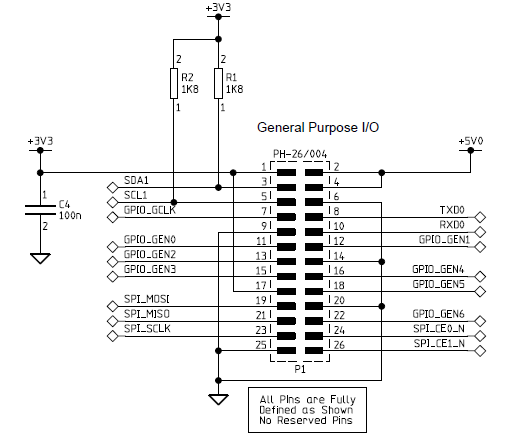
\includegraphics[width=0.7\textwidth]{Bilder/Schaltung_GPIO.png}
\end{figure}

Beim Raspberry Pi erf�llt jede GPIO Pin eine bestimmte Aufgabe. Einige Pins haben Doppelfunktionen. Alle Signale werden vom BCM2835 bereitgestellt. Die GPIO-Schnittstelle des Raspberry Pi Modell B, welches sic h in der Abbildung 3.1auf der oberen linken Ecke des Raspberry Pis befindet, besteht aus zwei Reihen mit jeweils 13 Pins.


\subsection{LAN9512}
\label{sec:LAN9512}
Das in dieser Arbeit eingesetzte Raspberry Pi Model B hat einen LAN9512. Der LAN9512 ist neben den SoC BCM2835 der zweite Chip auf dem Raspberry Pi Model B. Es beinhaltet verschiedene Einheiten, wie einen LAN-Controller und den USB Hub.

\begin{figure}[htbp]
	\caption{Prinzipschaltbild des LAN9512}
	\label{fig:LAN9512}
	\centering
		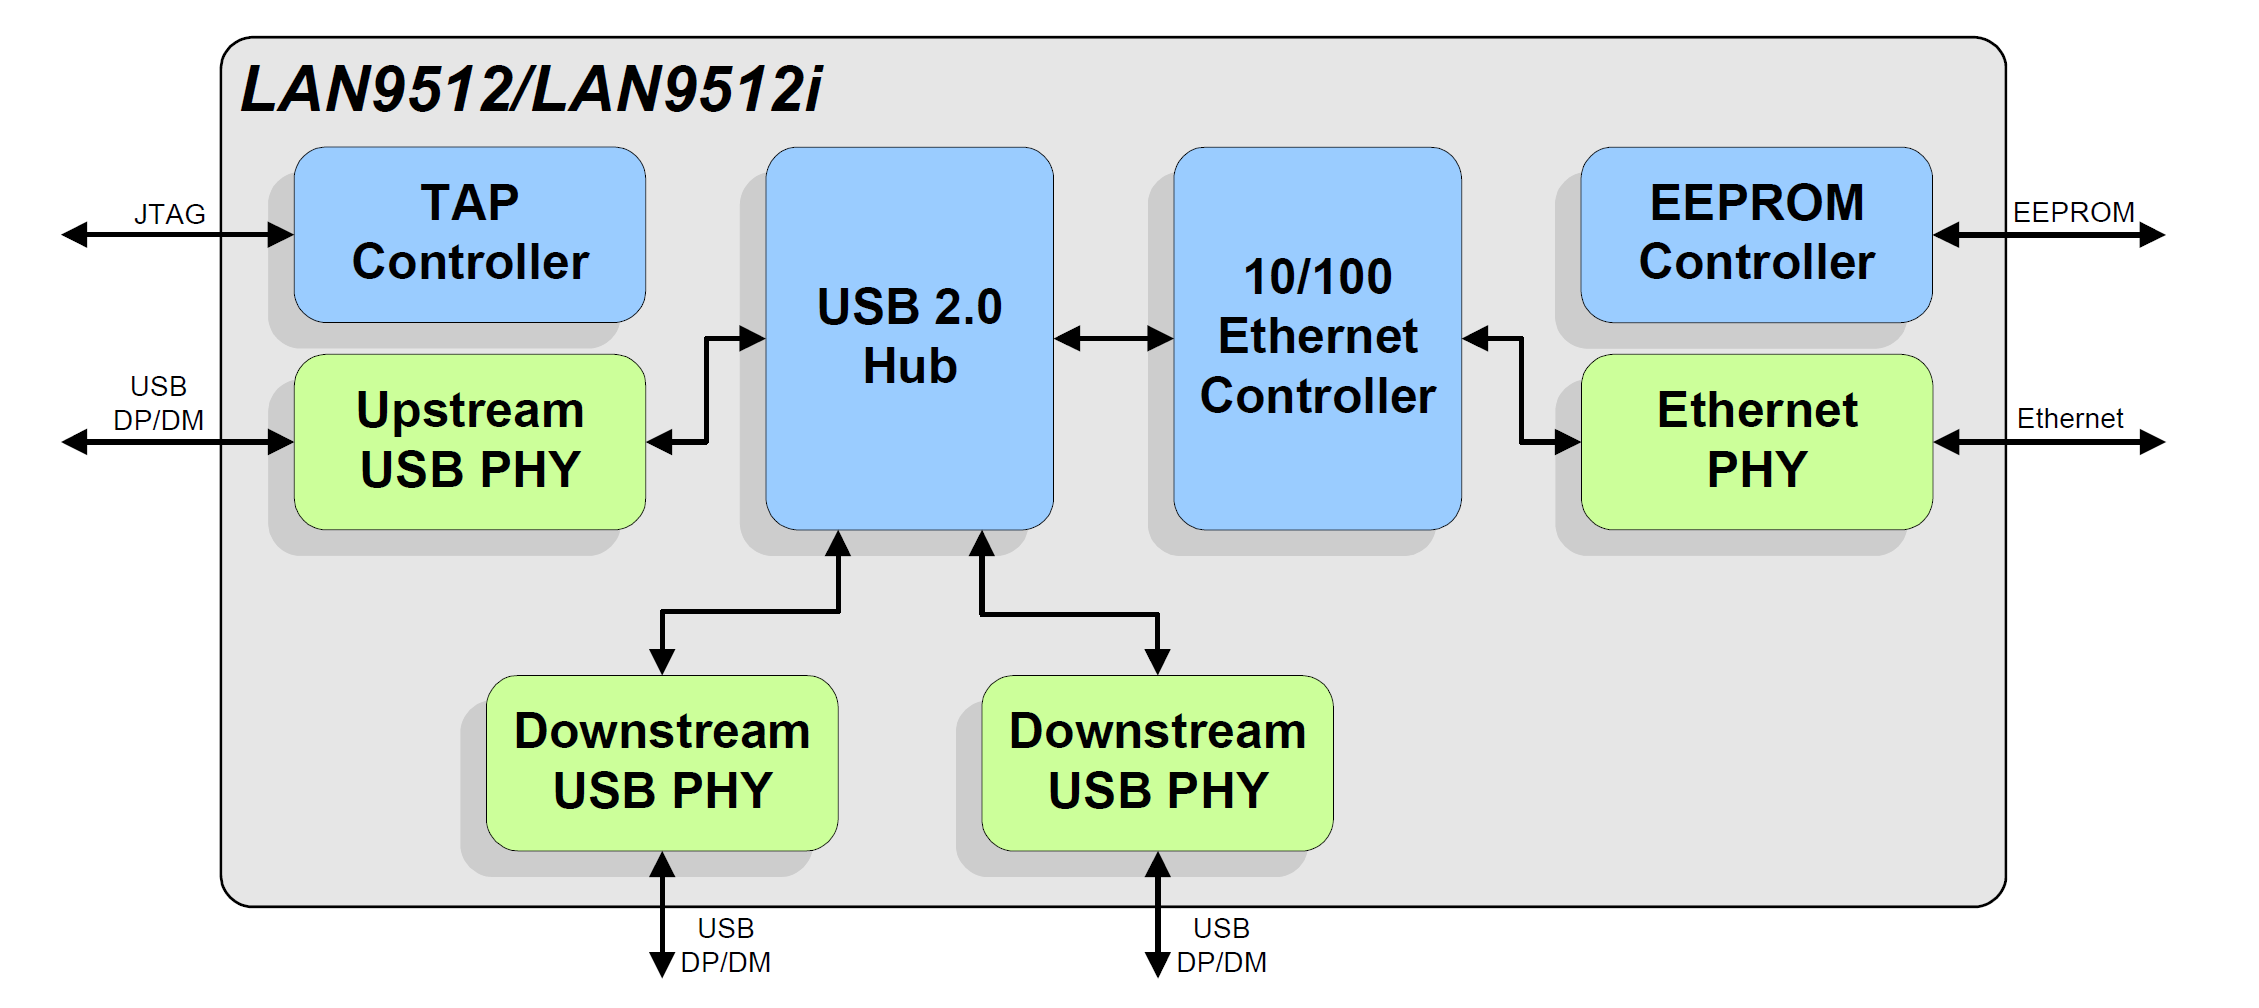
\includegraphics[width=0.70\textwidth]{Bilder/LAN9512.png}
\end{figure}

Anzumerken ist, dass der SoC BCM2835 als USB-Controller und der LAN9512 nur als USB-Hub mit 2 Ports dient [vgl. LAN9512, S. 6 und Dem2013, S. 81].
Der USB-Anschluss wird in dieser Arbeit nicht verwendet. Aber jedoch der Ethernet-anschluss.


\subsection{Ethernet}
\label{sec:Ethernet}

Der im LAN9512 eingesetzte Ethernet-Controller unterst�tzt die Ethernet-Standards
10Base-T mit 10Megabit/s, die im IEEE802.3 und 100Base-TX mit 100Megabit/s, welches
im IEEE 802.3u spezifiziert sind [vgl. LAN9512 S.7 und Dem2013 S.84]. Zus�tzlich
besteht die Funktion "`Wake on LAN"'. Dies bedeutet, dass der Raspberry Pi �ber das
angeschlossene Netzwerk aktiviert werden kann, wenn sich dieser im Ruhe Modus befindet.
100Base-TX unterst�tzt die automatische Detektion (Auto Negotiation) der Betriebsart.
Es erkennt also die Verdrahtung des Ethernet-Kabels, das an der RJ45-Buchse angesteckt ist.
Es wird auch Full-Dublex unterst�tzt, es kann somit gleichzeitig ge-sendet und empfangen werden [vgl. Dem2013 S.84]. 
\begin{figure}[htbp]
	\caption{Ethernet-Schaltung des Raspberry Pi Model B}
	\label{fig:RJ45_Anschluss_mit_LAN2512}
	\centering
		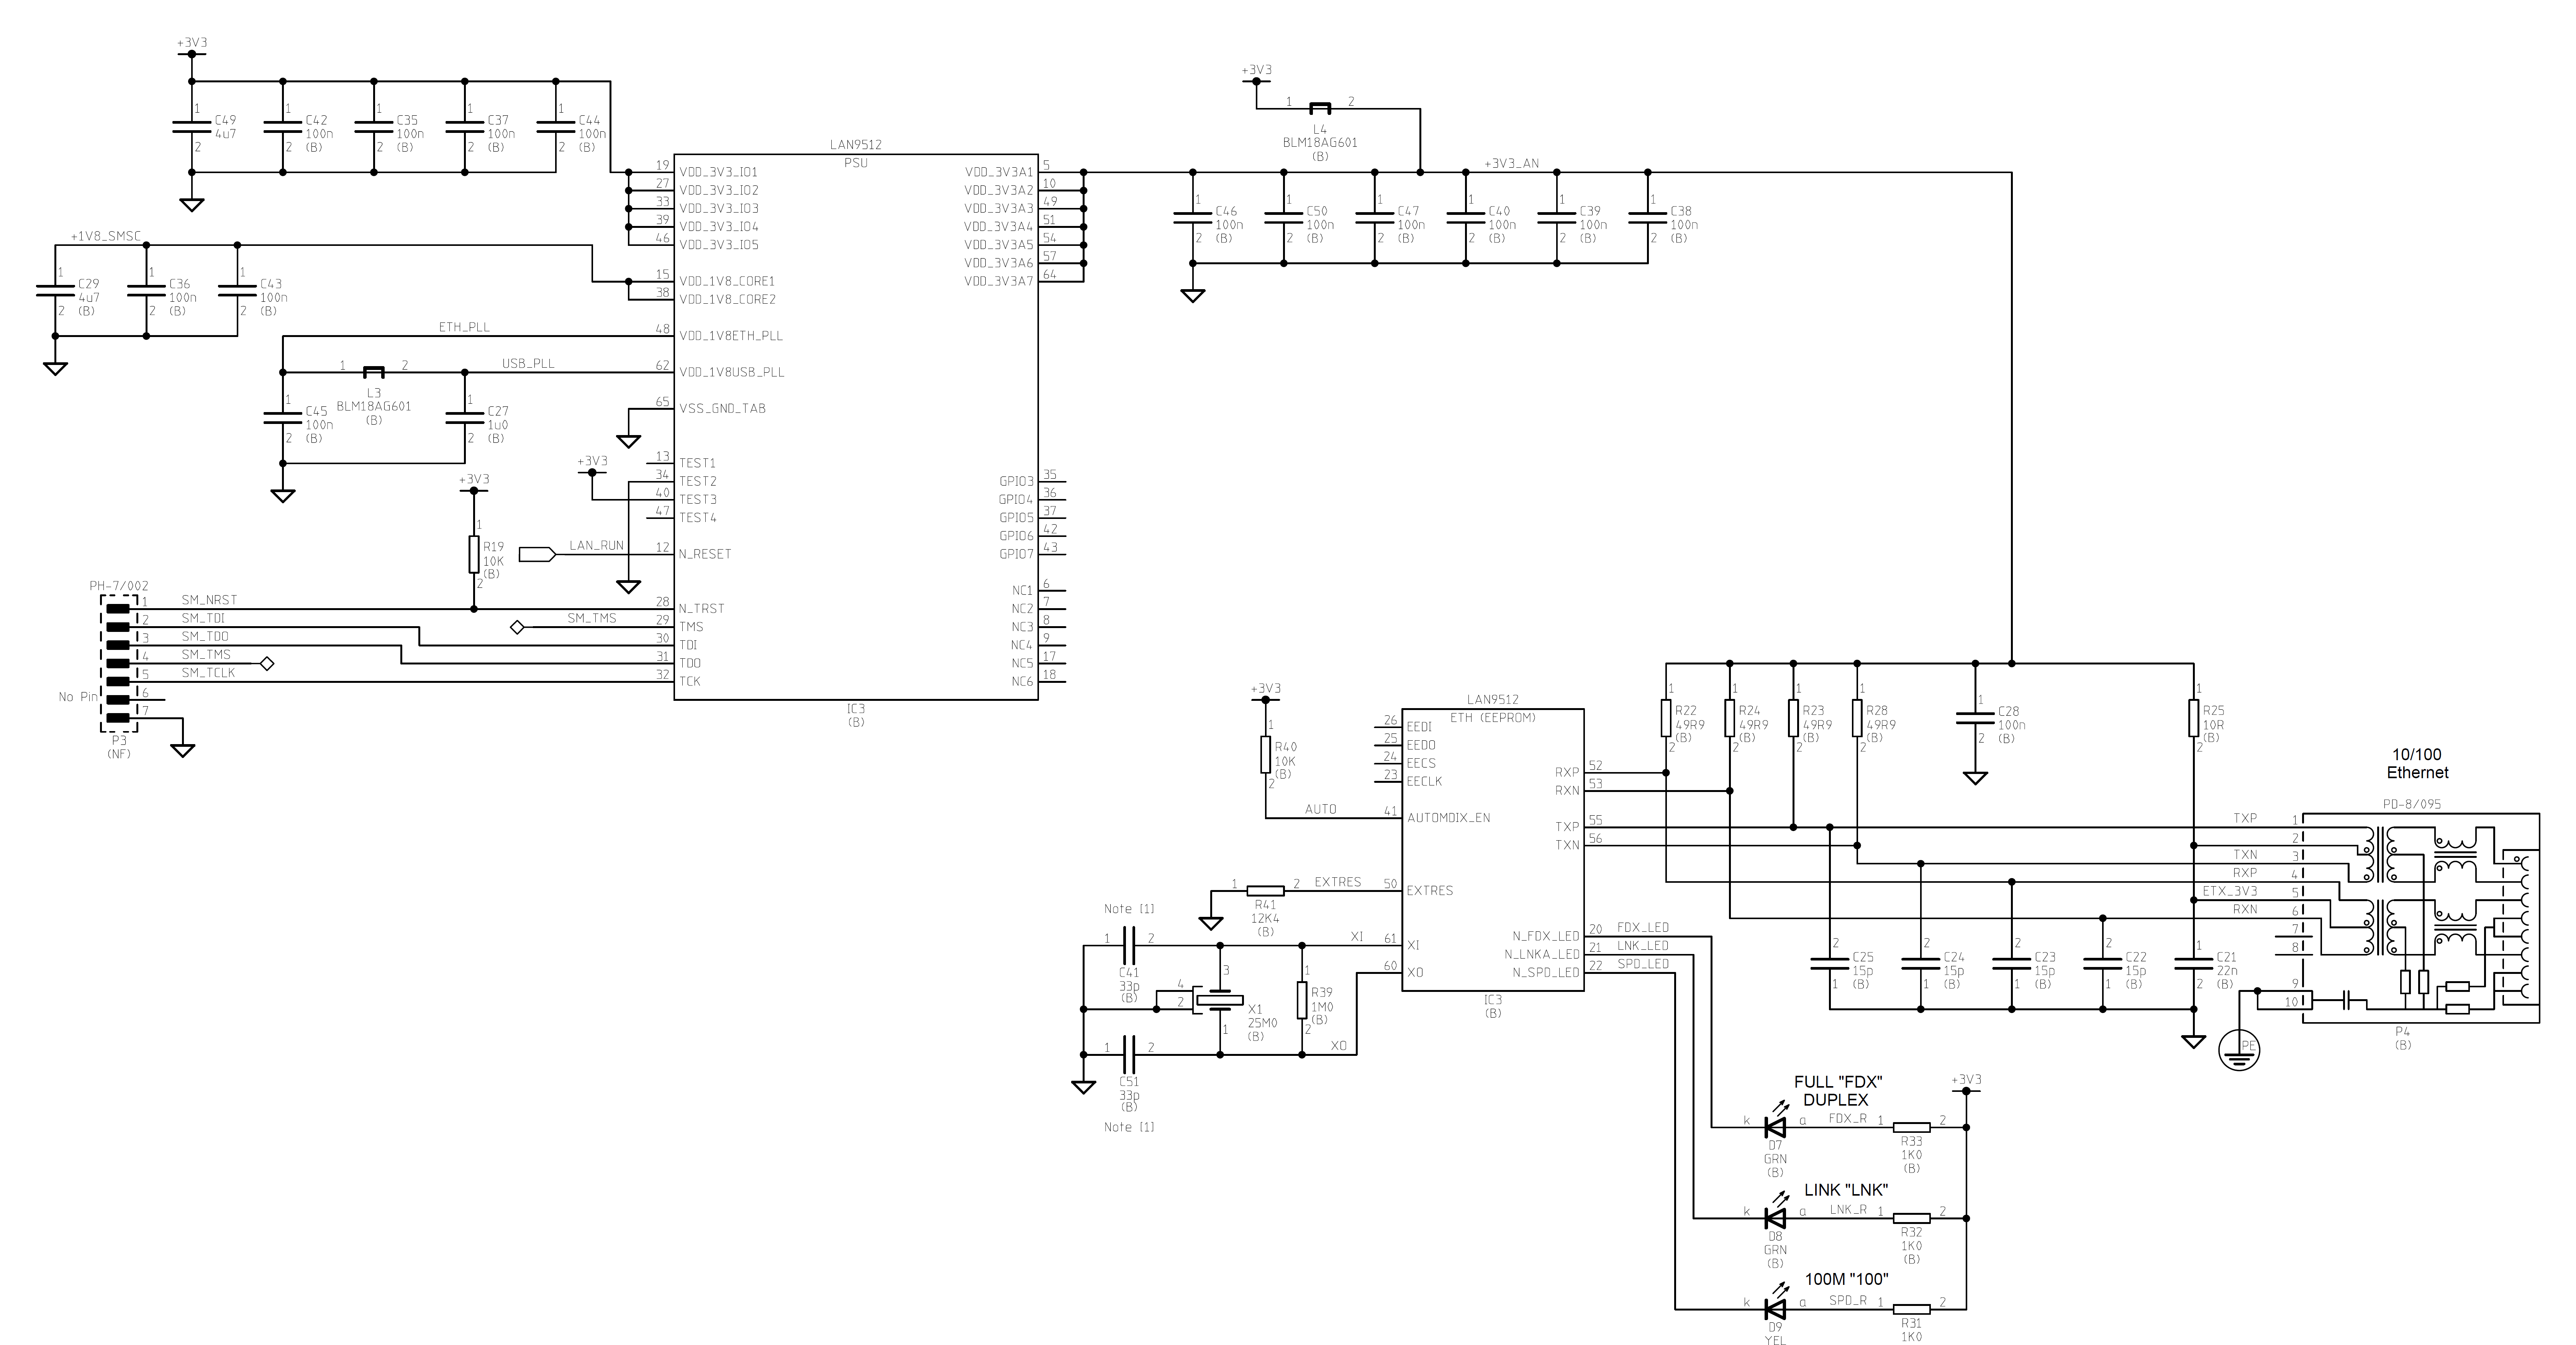
\includegraphics[width=0.80\textwidth]{Bilder/RJ45_Anschluss_mit_LAN2512.png}
\end{figure}



\section{Datenbusse}
\label{sec:Datenbusse}
Der Raspberry Pi Modell B stellt verschiedene Bussysteme zur Verf�gung. Bussysteme,
auch als Bus abgek�rzt, werden f�r die Daten�bertragung zwischen verschiedenen Teilnehmern
benutzt \cite[vgl.][S. 455]{Kof2015}. Je nach verwendetem Bussystem werden die
Daten seriell, also hintereinander �ber dieselben Datenleitungen oder parallel,
also gleichzeitig �ber verschiedenen Datenleitungen �bertragen. Auf dem Raspberry
Pi Modell B sind folgende f�nf Bussysteme verf�gbar, bei dem alle Daten seriell
�bertragen werden \cite[vgl.][S. 455]{Kof2015},

\begin{itemize}
	\item UART, Abk. f�r Universal Asynchronous Receiver/Transmitter.
	\item SPI, Abk. f�r Serial Peripheral Interface
	\item I$^{2}$C, Abk. f�r Inter Integrated Circuit
	\item I$^{2}$S, Abk. f�r Integrated Interchip Sound
	\item 1Wire, Eindraht-Verbindung.
\end{itemize}

Da in dieser Arbeit der UART und I$^{2}$C verwendet werden, werden diese zwei
Bussysteme beschrieben. Die vollst�ndige Erl�uterung der Bussysteme w�rde den
Rahmen dieser Arbeit sprengen, daher werden nur die grundlegenden Punkte erl�utert.
Die Bussysteme unterscheiden sich nicht nur, aber vor allem in der Daten�bertragung.
Dabei soll es zwei grunds�tzliche Formen der Daten�bertragung geben, die sich vor
allem bei der Synchronisation durch einen Takt unterscheiden \citealp[vgl.][S. 202 - S. 203]{Bei2011}:

Bei der \underline{synchronen Daten�bertragung} wird parallel zur Daten�bertragung der Takt
�bertragen. Durch die Takt�bertragung k�nnen die Kommunikationspartner den Be-ginn und das
Ende einer Daten�bertragung erkennen \cites[vgl.][S. 455]{Kof2015}[S. 202 bis S. 203]{Bei2011}.\\

Bei der \underline{asynchronen Daten�bertragung} existiert keine separate Taktleitung.
Die Daten werden als einzelne Zeichen �bertragen. Dabei werden diese in Start- und Stoppbits
verpackt. Die Start- und Stoppbits k�nnen variieren \cites[vgl.][S. 203]{Bei2011}.\\

Der Vollst�ndigkeit halber wird im Folgenden der 1Wire und I$^{2}$S beschrieben.
Beim 1-Wire Bus handelt es sich um einen Eindraht-Bus, deshalb auch der Name des
Bussystems \cite[vgl.][S. 491]{Kof2015}. Der, urspr�nglich vom Unternehmen Dallas (heute Maxim)\cite[vgl.][S. 3]{Gei}
entwickelte 1-Wire-Bus besitzt im Vergleich zu SPI und I$^{2}$C keine zus�tzliche Taktleitung.
Dabei handelt es sich also um eine asynchrone Daten�bertragung. 1-Wire-Bus f�hrt lediglich
neben der einzelnen Leitung zur Bus-kommunikation, also der Datenleitung mit der
Bezeichnung DQ, noch die Masse Lei-tung [vgl. Gei S. 3 und Kof2015 S.491]. Die Datenleitung
wird nicht nur dazu benutzt, um Daten zu senden und zu empfangen, sondern auch
um die Erweiterungen mit ei-ner Versorgungsspannung von 3,3 Volt zu versorgen [vgl. msx und Kof2015 S.491].
Die �bertragung erfolgt dabei seriell, bidirektional und asynchron, da �ber die Datenleitung
entweder nur gesendet oder empfangen werden kann und dies auch ohne Taktleitung erfolgt [vgl. Gei S. 3].

Der Raspberry Pi bietet ab der Revision 2 den Soundbus I$^{2}$S, Abk. f�r Integrated Interchip Sound.
Der I$^{2}$S Bus transportiert Audiosignale zwischen integrierten Schalt-kreisen. [vgl. Kof2015 S.489].

Das urspr�nglich von Motorola entwickelte Bussystem Serial Peripheral Interface (SPI)
arbeitet nach dem Master-Salve-Prinzip, mit einem Master und einer theoretisch unbegrenzten
Anzahl an Slaves. Dabei erfolgt die Kommunikation Synchron [vgl. Bei2011 S. 208].\\

\subsection{UART}
\label{sec:UART}

Der Universal Asynchrounous Receiver/Transmitter (kurz UART) Protokoll wird bei der Kommunikation von
RS232- oder RS485-Schnittstellen eingesetzt. Der UART wird auch zur Daten�bertragung mit 
Mikrocontrollern und wie hier mit Einplatinen-Computern benutzt.

Die Daten werden beim UART, im Gegensatz zum USART, der eine synchrone Daten�bertragung erlaubt,
asynchron �bertragen. Das hei�t dass es keine Taktleitung gibt. Der UART besitzt im Ruhezustand einen
High-Pegel, was der logischen 1 ent-spricht. [vgl. Pla uart] Die Daten werden mit einem Start- und
Stoppbit versehen. Es kann zus�tzlich einen Parit�tsbit geben.  �blicherweise werden acht bis neun Bits 
�bertragen [vgl. MUA]. Dabei werden also insgesamt 10 bis 12 Bits zusammen �ber-tragen. Diese werden 
auch als Wort bzw. Datenwort bezeichnet. Die Reihenfolge der �bertragenen Bits sieht beim UART 
folgenderma�en aus:

\begin{table}[htbp]
	\centering
	\caption{Aufbau des UART-Datenwortes}
	\label{tab:AufbauDesUARTDatenwortes}
		\begin{tabular}{|c|c|c|c|c|c|c|c|c|c|c|c|}
		\hline
		Startbit & D0 & D1 & D2 & D3 & D4 & D5 & D6 & D7 &\cellcolor[rgb]{1,1,0}{(D8)}&\cellcolor[rgb]{1,1,0}{(Parit�tsbit)}& Stoppbit \\ \hline
		\end{tabular}
\end{table}

Bei der obigen Abbildung zum Aufbau des UART-Datenwortes ist jedes K�stchen f�r ein Bit gedacht. Der Startbit wird als eine Logische 0 gesendet [vgl. Pla uart]. Zwischen zwei Datenworten k�nnen sich beliebig lange Pausen befinden, da jedes Wort am Startbit erkannt wird [vgl. Pla uart]. Die Bits D8, also der neunte Datenbit und die Parit�tsbits sind gelb hintermalt, da diese optional sind.

Das Parit�tbit �berpr�ft, ob die Daten richtig �bertragen wurden. Dabei wird zwischen
odd parity und even parity unterschieden. Bei odd parity wird der Parit�tsbit auf eins
gesetzt, wenn es in den Datenbits eine gerade Anzahl an Einsen gibt [vgl. M�l2009 S. 6].

Even parity bildet den Gegensatz zur odd parity. Bei einer geraden Anzahl von Datenbits
wird das Parit�tsbit auf Null und bei einer ungeraden Anzahl auf eins gesetzt [vgl. M�l2009 S. 6].

Beim Stoppbit muss erw�hnt werden, dass auch zwei Stoppbits hinter ein Daten-wort eingef�gt
werden k�nnen, um den Pausenpegel zwischen zwei Datenworten bei der �bertragung zu trennen
[vgl. Bei2011 S. 262]. Da die Kommunikation beim UART asynchron abl�uft synchronisieren
sich die Kommunikationsteilnehmer f�r jeden Transfer neu [vgl. Pla uart]. Dies geschieht
durch die oben erw�hnten Start- und Stoppbits. Vor der Daten�bertragung liegt der Pegel auf
der �bertragungsleitung auf high [vgl. Pla uart]. Das bedeutet, dass die Leitung sich auf 3,3 Volt befindet.

Vor der Kommunikation zwischen Sender und Empf�nger m�ssen diesen die Anzahl der
Datenbits, Startbits und der Stoppbits sowie der Berechnung der Parit�t und die Frequenz
des �bertragungstaktes der Daten kenntlich gemacht werden. Soll et-was �bertragen werden,
wird dies dem Empf�nger der Daten durch den Startbit kenntlich gemacht. Anhand des
High-Low-Pegels wird der Sendevorgang kenntlich gemacht, wodurch Empf�nger und Sender
synchronisiert sind. Der Sendevorgang wird durch einen Stoppbit beendet [vgl. Pla uart].
Der UART am Raspberry Pi besitzt die Leitungen TxD (am Pin 8) zum Senden und RxD (am Pin 10)
zum Empfangen der Daten [vgl. Upt2014 S. 222]. Das Raspberry besitzt keine Leitung f�r einen
Hardware-Handshake [vgl. Pla uart], zur Erkennung der �bertragung. Wird ein hardwarebasierter
Handshake ben�tigt, kann auf einen freien GPIO-Pin zugegriffen werden [vgl. Pla uart].

Ein Baudratengenerator bzw. programmierbarer Timer sorgt f�r die �bertragungsgeschwindigkeit,
auch Baud oder Baudrate genannt, der Daten [vgl. Bei2011 S. 262]. Die Baudraten
m�ssen sowohl auf Empf�ngerseite als auch auf der Senderseite �-bereinstimmen,
da die Daten sonst nicht korrekt �bertragen werden k�nnen. Das hat den Hintergrund,
dass der UART - wie oben erw�hnt - keine Taktleitung hat und der Empf�nger nicht wei�,
wann �ber UART Daten geschickt werden und wann nicht.


\subsection{I$^{2}$C}
\label{sec:I2C}

Das im Jahre 1982 von Philips Semiconductor entwickelte Bussystem Inter Intergratet Circuit (I$^{2}$C)
wird f�r die Verbindung von integrierten Schaltungen auf Platinen bzw. innerhalb von Ger�ten
eingesetzt [vgl. Bei2011 S. 209 und Dem2013 S. 185]. Beim I$^{2}$C handelt es sich um eine
serielle Schnittstelle [vgl. Dem2013 S. 185], bei der die Daten�bertragung sowohl synchron
als auch asynchron erfolgt [vgl. Bei2011 263 bis S. 264].\\

Das Bussystem kann mit zwei bzw. drei Leitungen eingesetzt werden. Eine Leitung dient als
Taktleitung, eine zweite als Datenleitung, wobei die dritte Leitung die Mas-seleitung ist,
die als Bezugspegel dient [vgl. Bei2011 S. 209]. I$^{2}$C besitzt keine sepa-rate Leitung zum
Ausw�hlen der einzelnen Teilnehmer. Die einzelnen Teilnehmer werden durch Adressen
ausgew�hlt [vgl. Kof2015 S.476]. Beim Raspberry Piwird der I$^{2}$C Datenbus auch vom BCM2835,
also dem SoC, bereitgestellt [vgl. Upt2014 S. 223]. Der I$^{2}$C besitzt folgende Leitungen:

\begin{description}
	\item[SDA Serial Data- Line] hier�ber werden die Daten zwischen den Kommunikationspartnern �bertragen 
	\item[SCL Serial Clock Line] Taktleitung des Bussystems
\end{description}

Die �bertragung der Daten erfolgt aus einer Mischung aus synchroner als auch asynchroner �bertragung. Das bedeutet, dass bei der �bertragung der einzelnen Datenpakete diese jeweils mit Start und Stoppbits versehen werden [vgl. Bei2011 263 bis S. 264]. Die �bertragung der einzelnen Bits der Datenpakete wird jedoch mit dem Taktsignal der SCL-Leitung des jeweiligen Masters synchronisiert �bertragen [vgl. Bei2011 S. 264].\\

An das Bussystem k�nnen ein oder mehrere Master angeschlossen werden, von denen jedoch mindestens einer die Kommunikation innerhalb des I$^{2}$C steuert [vgl. Bei2011 S. 209]. Ein Bus, der mehrere Master besitzt, wird auch als Multimasterbus bezeichnet [vgl. Dem2013 S. 187]. Am Bus k�nnen bis zu 128 Slaves angeschlossen werden, die eine im Bussystem eindeutige Adresse von sieben bzw. zehn Bit L�nge besitzen [vgl. Dem2013 S. 189], wodurch die Slaves einzeln angesprochen werden k�nnen [vgl. Bei2011 S. 209 bis 210]. Die 10 Bit Adressierung soll kaum genutzt werden [vgl. Dem2013 S. 189]. Die Slaves k�nnen dadurch immer zum Senden bzw. Empfangen von Daten durch den Master aufgefordert werden. Der Empfang der Auf-forderung wird dem Master durch ein Quittierungsbit (auch Acknowledge bezeichnet) best�tigt [vgl. Bei2011 S. 210].\\

Da I$^{2}$C-Busse in der Regel Open-Collector-Eing�nge besitzen, versorgen die
I$^{2}$C-Bausteine keine Spannungspegel an ihren Pins. Beim Raspberry Pi werden
die I$^{2}$C Pins jedoch durch Pull-Up-Widerst�nde auf 3,3 Volt gezogen, dieser
bildet dann den positiven Signalpegel [vgl. Bei2011 210]. Bei der Kommunikation
�ber die I$^{2}$C- Schnittstelle werden diese Leitungen auf Masse gezogen [vgl. Kof2015 S.476],
das bedeutet, dass diese Leitungen dann auf 0 Volt herunter gezogen werden und
somit auch einen LOW-Pegel besitzen [vgl. Kof2015 S.476].

\begin{table}[htbp]
	\centering
	\caption{Aufbau des UART-Datenwortes}
	\label{tab:AufbauDesUARTDatenwortes}
		\begin{tabular}{|c|c|c|c|c|c|c|c|c|c|}
		\hline
		Start & Slave & Adresse & Read/Write & Ackn. & Daten & Ackn. &  Daten & Ackn. & Stop \\ \hline
		\end{tabular}
\end{table}

In der Abbildung befindet sich der Startbit ganz links und der Stoppbit ganz rechts.
Beim "`Ackn."' handelt es sich um den Quittierungsbit, was nach jeder Daten�bertragung vom Slave an den Master erfolgt.

Beim I$^{2}$C kann jede Baugruppe, je nach Funktion, entweder als Sender oder als
Empf�nger arbeiten. Dabei k�nnen mehrere Master im System existieren. Die Erzeugung
des Taktes erfolgt immer durch den Master, wobei jeder Master seine eige-ne Taktfrequenz
besitzt [vgl. Dem2013 S. 187 bis S. 188].

\begin{figure}[htbp]
	\caption{Prinzipielles Aufbau des I$^{2}$C Datenformates}
	\label{fig:I2C_Datenuebertragung}
	\centering
		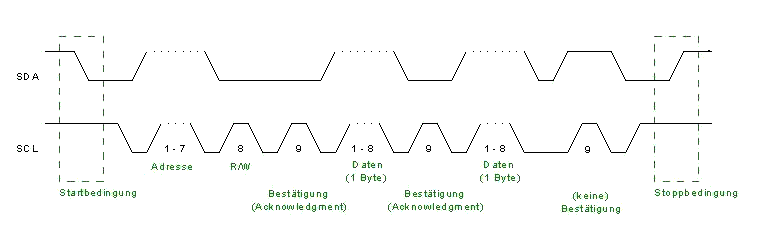
\includegraphics[width=1.00\textwidth]{Bilder/I2C_Datenuebertragung.png}
\end{figure}
Da der Bus vom Raspberry Pimit einer Spannung von 3,3 Volt versorgt wird, befinden
sich die Leitungen SDL und SCL im High-Pegel wenn keine Busaktivit�t stattfin-det [vgl. Kof2015 S.476].
Es hat also den logischen Wert 1. Sollen Daten �bertragen werden geht das Datensignal
SDA von High auf Low �ber, gleichzeitig befindet sich jedoch die Taktleitung auf High.
Dabei handelt es sich um den Startbit. Der Startbit ist in der Abbildung 3.8 auf der
linken Seite umrahmt. Im Gegensatz dazu bildet der Stoppbit einen Low zum High-�bergang
des SDL bei gleichzeitigem High Pegel der Taktleitung. Dieser ist in der Abbildung 3.8
auf der rechten Seite umrahmt [vgl. rni].

Mit der Slave Adresse, die in der Regel sieben Bit gro� ist, wird das jeweilige Slave
Bauelement des I$^{2}$C angesprochen. Der Read/Write Bit gibt die Richtung der
Daten�bertragungen an. Bei Read (logische 1), liest der Slave ein und bei Write (logische 0),
schreibt der Slave. Die Richtung der Daten�bertragung wird vom Slave an den Master gemeldet [vgl. rni und Dem2013 S. 189].

Bei der Kommunikation �ber den I$^{2}$C erfolgt die Best�tigung, also der Quittierungsbit
(in der Abbildung 3.8 als "`Ackn."' dargestellt), f�r die �bertragungsrichtung
durch den Slave. Bei der Daten�bertragung an sich best�tigt der Empf�nger der Daten
dem Sender den Empfang der Daten. Falls der Slave die Daten empf�ngt, setzt der Master
den SDA auf High und erwartet vom Slave, dass dieser den SDA auf Low zieht. Geschieht
das nicht, wird die �bertragung gestoppt. Im umgekehrten Fall, wenn der Master der Empf�nger
ist, setzt der Slave den SDA auf High, falls es nicht best�tigt wird, erfolgt der
Abbruch der Daten�bertragung [vgl. Dem2013 S. 189]. Die Best�tigung muss innerhalb
von neun Takten des jeweiligen Masters erfolgen [vgl. rni]. Bei der Daten�bertragung
an sich muss der Takt selbst High sein, wenn ein Bit �bertragen wird und dieser als
g�ltig gelten soll [vgl. rni].

Auf dem Raspberry Pi existieren zwei I$^{2}$C-Schnittstellen [vgl. Upt2014 S. 223].
Der erste befindet sich in der GPIO-Schnittstelle mit der Bezeichnung P1. Der zweite
bestimmt ist [vgl. Upt2014 S. 223]. Der Aufbau der zweiten I$^{2}$C Schnittstelle wird
befindet sich an der GPIO Schnittstelle P5, welcher nicht f�r den allgemeinen Gebrauch
am Anfang der Kapitels GPIO-Anschl�sse beschrieben. Die erste I$^{2}$C Schnittstelle
kann �ber die GPIO-Schnittstelle mit der Bezeichnung P1 �ber zwei Pins benutzt werden.
Dazu dient der Pin 3 als SDA, also als Datenleitung und der Pin 5 als SCL, also um den
Takt f�r die Synchronisation der Kommunikation zu �bertragen. Die Pins sind mit zwei
Pull-Up-Widerst�nden verschaltet [vgl. Dem2013 S. 188].

Der I$^{2}$C arbeitet nach dem Master-Slave Prinzip. Beim Master handelt es sich um
die aktive Komponente, beim Slave um die passive. Der Master steuert also die gesamte
Kommunikation, sodass die Slaves lediglich auf die Anfragen des Masters an-sprechen m�ssen.




\section{Beschreibung des Aufsatzes SD0}
\label{sec:BeschreibungDesAufsatzesSD0}

Beim Aufsatz handelt es sich um eine Erweiterung f�r den Raspberry Pi. Aufs�tze
werden bei Raspberry Pi dazu verwendet, um diesen mit zus�tzlichen Funktionalit�ten
auszustatten oder zu erweitern.

Bei der benutzten Erweiterung handelt es sich um den Aufsatz SD0 des Unternehmens
Busware. Der Aufsatz SD0 wird auf die als P1 bezeichneten General Purpose Input Output (GPIO)
Pins des Raspberry Pi aufgesetzt. Diese GPIO-Leiste des Raspberry Pi wird zur Erweiterung des
Raspberry Pi verwendet. Bei dieser Bachelo-rarbeit werden �ber den Aufsatz SD0
Energieverbrauchsdaten �ber dessen S0-Schnittstellen erfasst. Der SD0 wird verwendet,
da dieser durch die Aufgabenstel�lung vorgegeben ist. In diesem Kapitel wird der
Aufsatz SD0 beschrieben. Da der aktuelle Schaltplan nicht zur Verf�gung steht,
wird der SD0 basierend auf dem Schaltplan \emph{Version 1.1} beschrieben.

\subsection{S0-Schnittstellen des SD0}
\label{sec:S0SchnittstellenDesSD0}
Neben der Steckleiste, mit der der Aufsatz SD0 auf die GPIO Steckleiste mit der
Bezeichnung P1 des Raspberrry Pi aufgesteckt wird, besitzt der Aufsatz vier
S0-Schnittstellen, auch Chanels (engl. f�r Kanal) genannt, �ber die die Verbrauchsdaten
erfasst werden.

\begin{figure}[h]
	\centering
	\caption{S0-kan�le des SD0}
	\label{fig:busware_s0}
		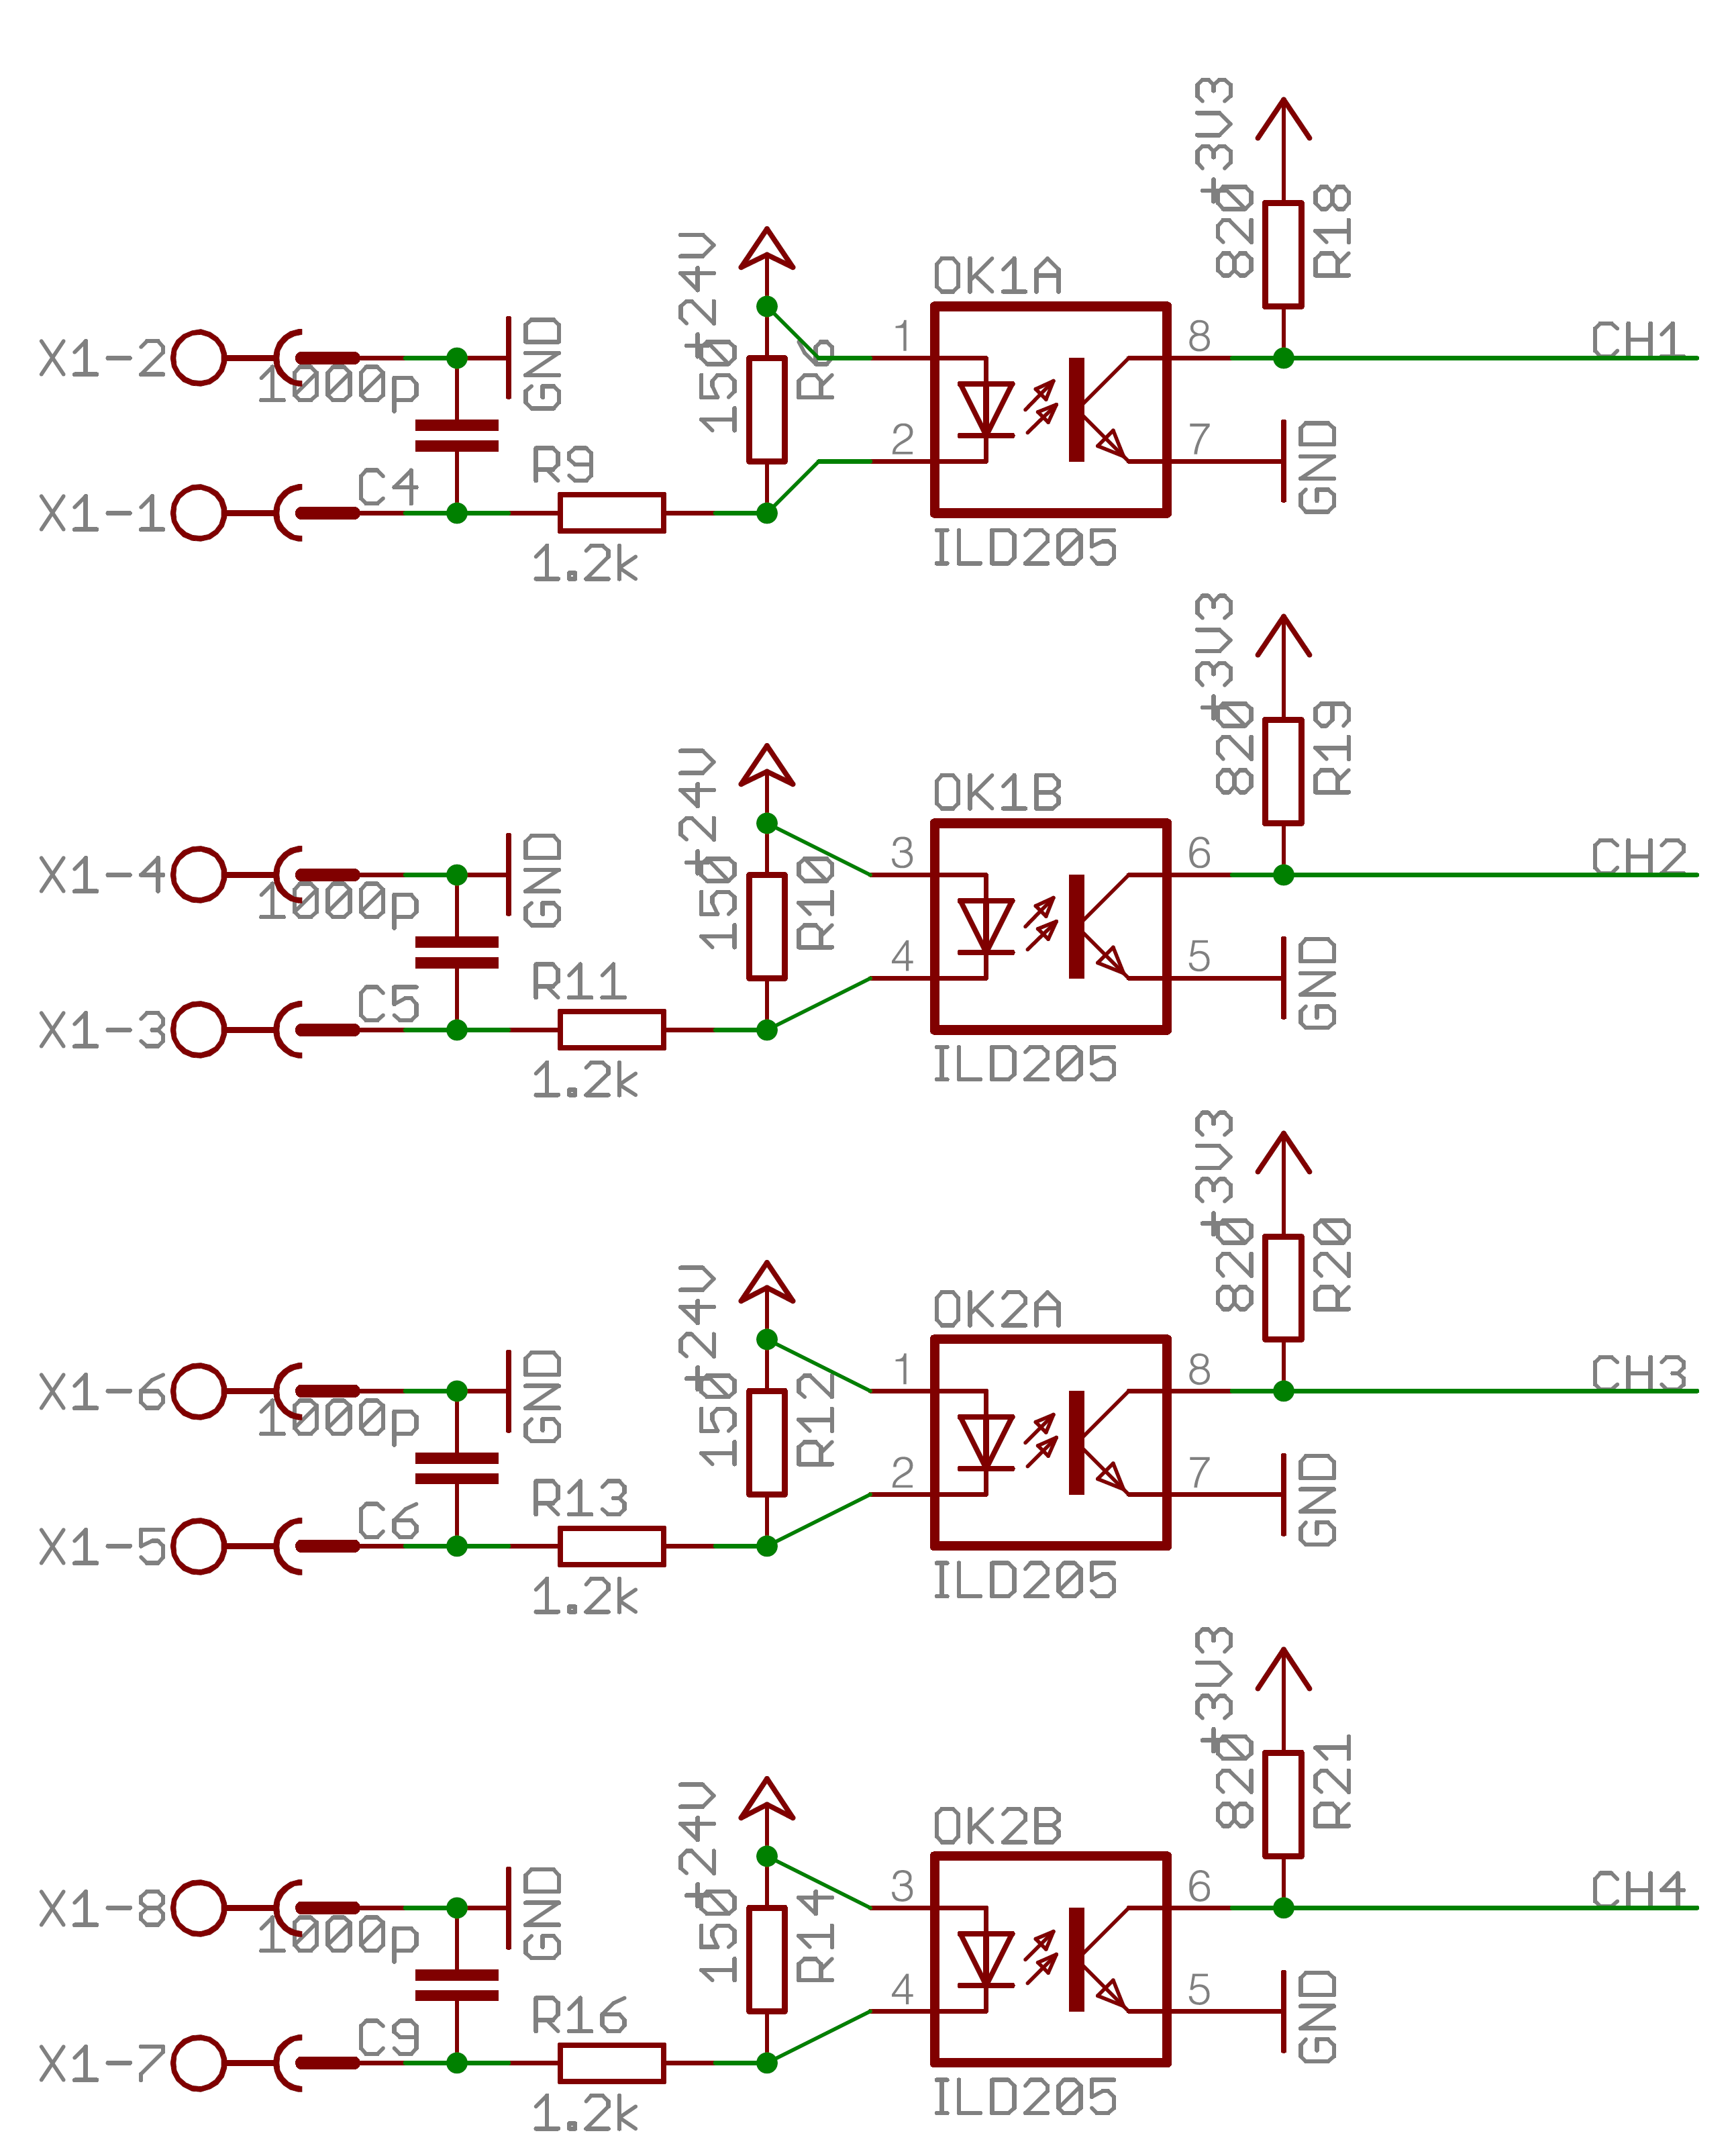
\includegraphics[width=0.60\textwidth]{Bilder/busware_s0.png}
\end{figure}

Zus�tzlich befindet sich eine RJ-10-Schnittstelle sich auf dem SD0. Daneben ist
die Erweiterung mit einem Mikrocontroller, dem Atmega1284p best�ckt. Dieser ist
mit der seriellen Schnittstelle RJ-10-Schnittstelle, den vier S0-Schnittstellen
nach DIN 43864 / EN 62053-31 und der Steckverbindungsleiste verbunden. Zus�tzlich
besitzt die Erweiterung eine Real Time Clock (RTS), die f�r Echtzeitanwendungen
oder hier dem Raspberry Pi zu gute kommen kann [vgl. bsd0 Specs].


\subsection{Real Time Clock (RTC)}
\label{sec:RealTimeClockRTS}

Bei Real Time Clock, kurz RTC bezeichnet, handelt es sich um Echtzeituhren die
Systemzeiten bereitstellen. RTCs stellen also Datum und Uhrzeit bereit [vgl. Bei2011 278].
Beim Real Time Clock des SD0 handelt es sichn um den DS1338U33. Da der Raspberry
Pi ohne einen Internetzugang seine Uhrzeit nicht abgleichen kann, bietet sich die
M�glichkeit an, die Uhrzeit beim RTC des SD0 zu beziehen. Wobei der RTC durch den
Atmega1284p dem Rasperry Pi bereitgestellt wird.

\begin{figure}[htbp]
	\caption{Echtzeituhr des SD0}
	\label{fig:RTC_SD0}
	\centering
		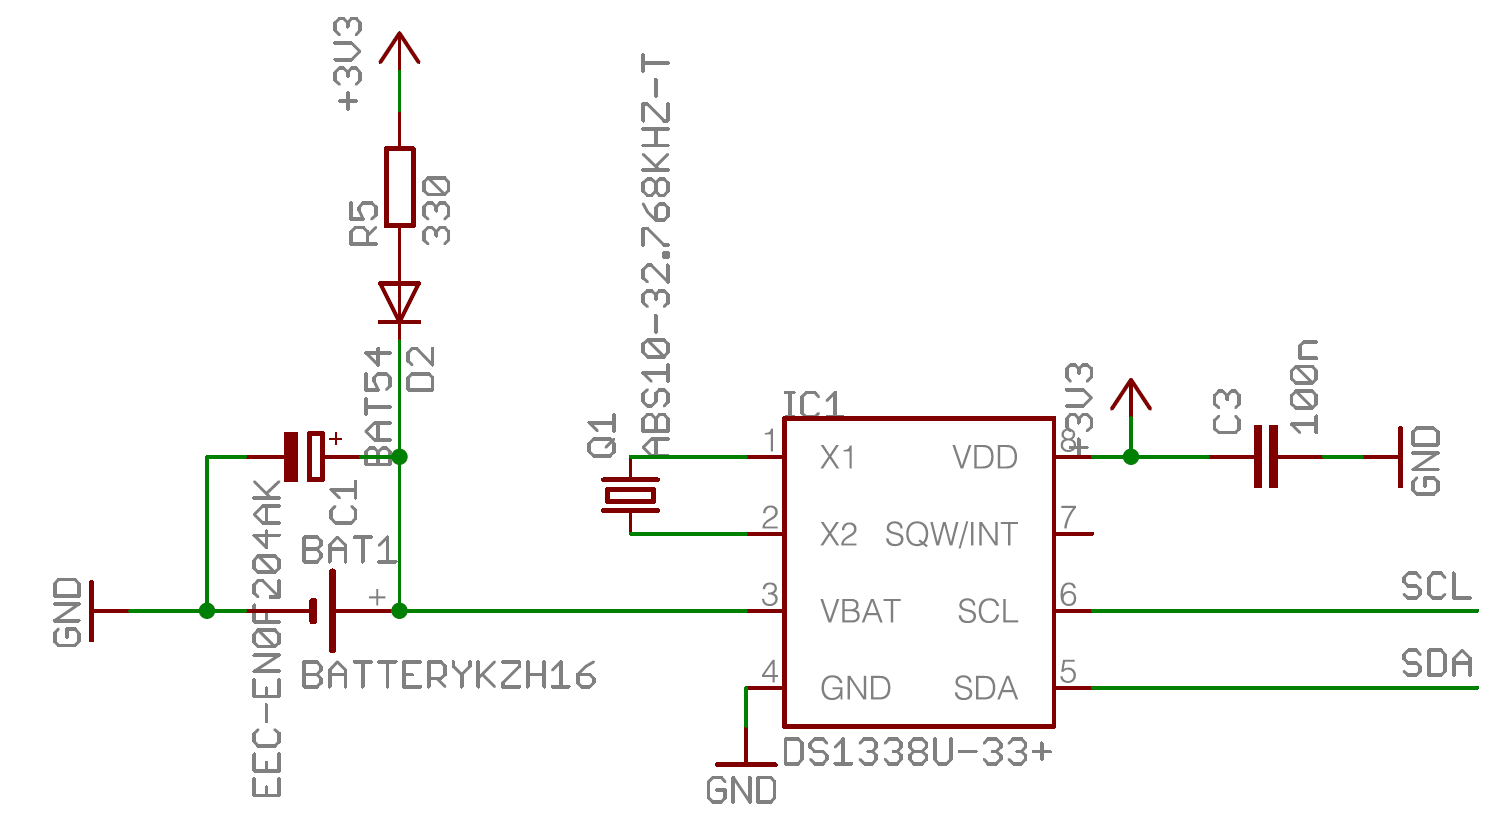
\includegraphics[width=0.70\textwidth]{Bilder/RTC_SD0.png}
\end{figure}

Die Verbindung zur Echtzeituhr wird �ber eine I$^{2}$C Verbindung erstellt. Daf�r
stehen wie in der Abbildung 3.1 dargestellte Leitungen SCL und SDA bereit, welche
jeweils als Takt- und Datenleitung des I$^{2}$C verwendet werden. Es bietet sowohl
die Uhrzeit in den Einheiten Sekunden, Minuten, Stunden als auch den Tag, Monat und
Jahr als Datum an. Die Uhrzeit wird entweder im 12 Stunden oder 24 Stunden Format
bereit-gestellt. Beim 12 Stundenformat indiziert es die AM/PM [vgl. DS1338 S. 1 General Description].
Die Monatsenden werden bei Monaten mit weniger als 31 Tage aut-matisch angepasst.
Es beinhaltet auch die Erkennung von Schaltjahren. Es besitzt einen Stromerkennungssensor.
Es schaltet auf einen 220 mF Kondensator um, wenn es mit zu wenig Strom versorgt wird. [vgl. DS1338 S. 1]


\subsection{Mikrocontroller des SD0}
\label{sec:MikrocontrollerDesSD0}
Neben dem im vorherigen Kapitel beschriebenen RTC ist der SD0 mit einem Mikrocontroller
best�ckt. Bei dem 8-Bit Mikrocontroller handelt es sich um den Atme-ga1284p. Der 8-Bit
Mikrocontroller basiert auf dem AVR. [atm1284 S. 3] �ber das Atmega1284p werden die an
den S0-Schnittstellen empfangenen Daten aufbereitet und an den Ausg�ngen bereitgestellt [bsd0 Specs].


\begin{figure}[htbp]
	\centering
	\caption{Mikrokontroller des SD0}
	\label{fig:SD0_Chanels}
		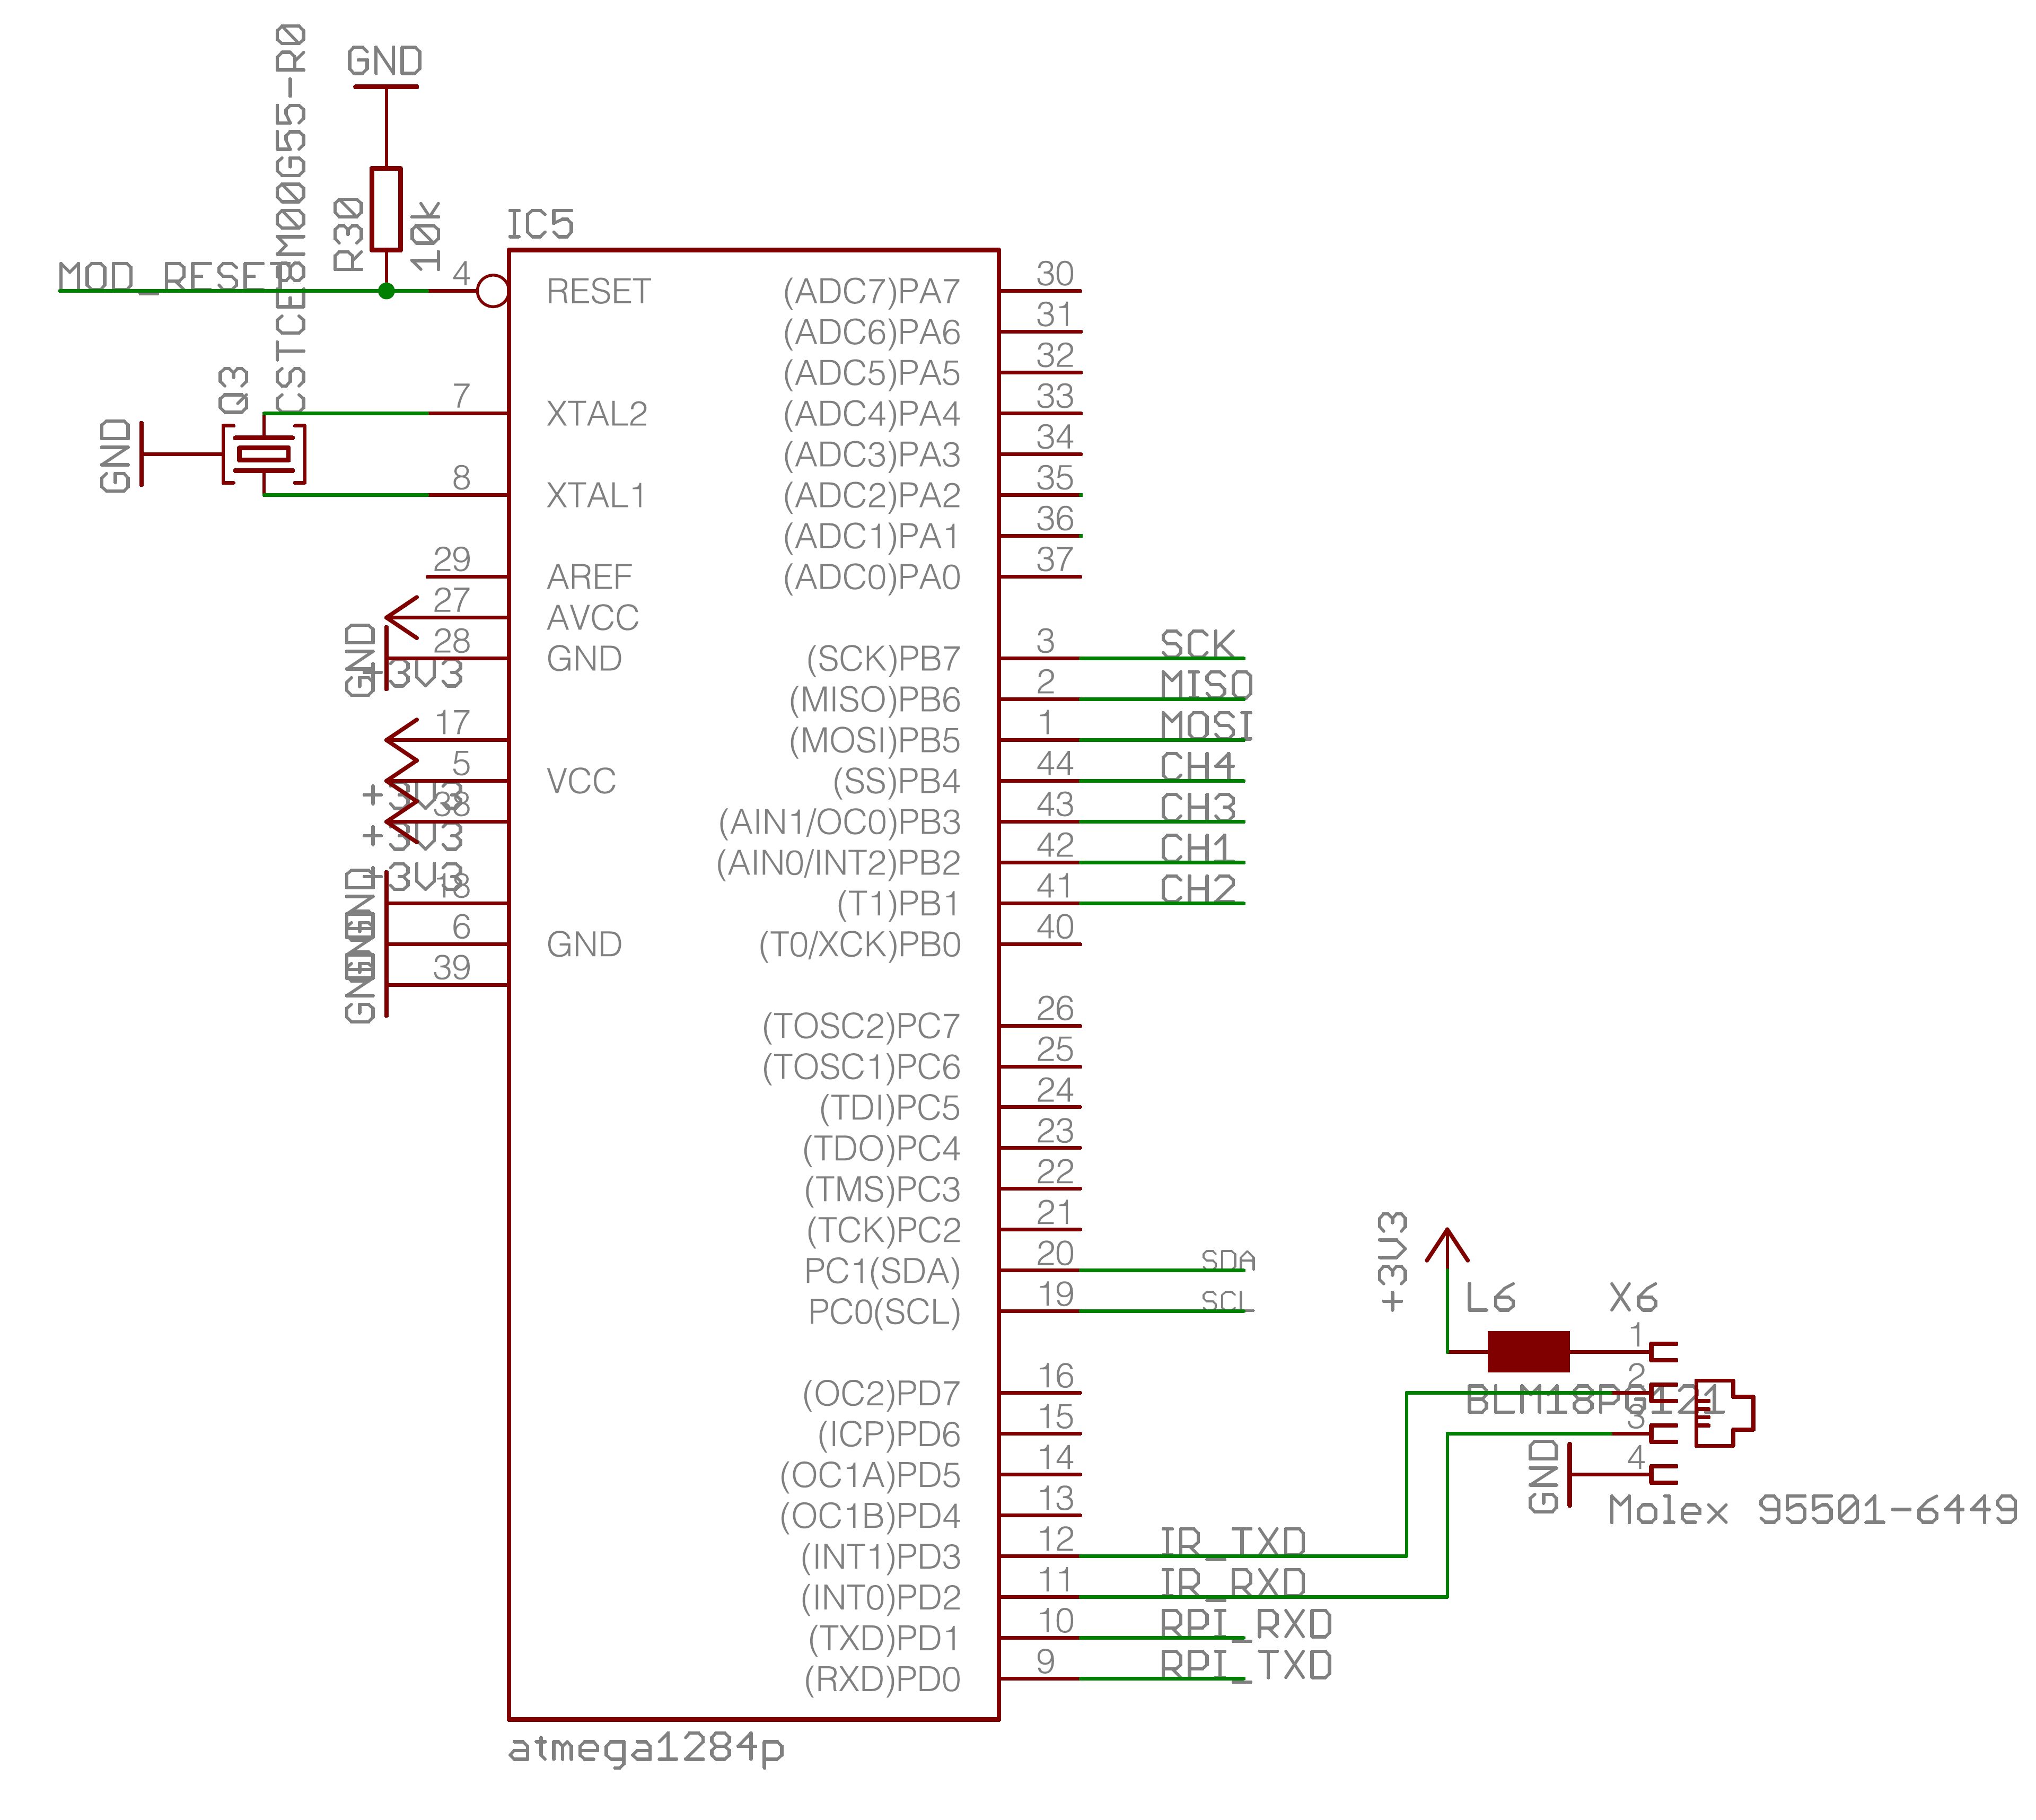
\includegraphics[width=0.50\textwidth]{Bilder/SD0_Chanels.png}
		\center
	\quelle{\cite{sad}}
\end{figure}

Wie der Raspberry besitzt der Atmega 1284p eine GPIO Schnittstelle, beim Amega1284p
besitzt sie jedoch 32 Pins. Durch den Atmega1284p wird auch das RTC bereitgestellt.
Der Mikrocontroller kann �ber zwei USART und eine SPI Schnittstelle kommunizieren. [atm1284 S. 4]



\section{S0-Schnittstelle}
\label{sec:S0Schnittstelle}
Die S0-Schnitstelle wird nach \textit{DIN EN 62053-31 definiert} und in der Geb�udeautomatisierung
verwendet. Die Schnittstelle wird in Elektrizit�tsz�hlern eingebaut. Mit
Impulseinrichtungen wie die S0-Schnittstelle werden Impulse, die der aktuell verbrauchten
Energiemenge entsprechen, an den Empf�nger �bertragen \cite[][][s0norm S.4].

\begin{figure}[htbp]
	\caption{S0-Schnitstelle in Stromz�hlern}
	\label{fig:S0Schnitstelle in Stromz�hlern}
	\centering
		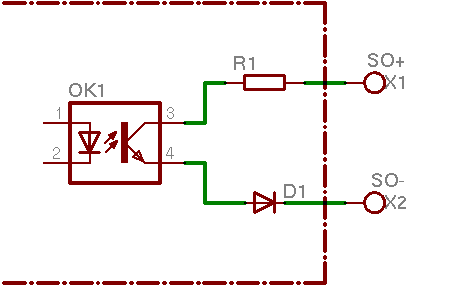
\includegraphics[width=0.40\textwidth]{Bilder/S0.png}
\end{figure}

Die Impulseinrichtungen geben eine bestimme Anzahl von Impulsen pro Wattstunde.
Dabei gibt es zwei Arten bzw. Klassen von Impulsausg�ngen [s0 norm S.5]:

\begin{description}
	\item[Impulsausgang der Klasse A:] �bertragung �ber gr��ere Entfernungen;
	\item[Impulsausgang der Klasse B:] geringe Entfernung und geringer Energieverbrauch
\end{description}

Dabei kann die Schnittstelle sowohl im Stromz�hler als auch im Gas- oder Wasserz�hler
eingesetzt werden. Bei der �bertragung von Messwerten wird f�r jedes
verbrauchtes Watt pro Stunde (Wph) ein gewichteter Impuls �bertragen. Die Gewichtung
des Impulses ist von Z�hler zu Z�hler unterschiedlich [vgl. S0S]. F�r die zwei
Arten bzw. Klassen von Impulsausg�ngen sind den Impulsen verschiedene Grenzen
gesetzt:

\begin{table}[!htbp]
	\centering
	\caption{S0-Schnitstelle in Stromz�hlern}
	\label{tab:S0SchnitstelleInStromz�hlern}
	
		\begin{tabular}{|c|c|c|}
				\hline
				
				Parameter & \multicolumn{1}{c|}{\begin{tabular}[c]{@{}c@{}}Impulseinrichtung\\ der Klasse A\end{tabular}} & \multicolumn{1}{c|}{\begin{tabular}[c]{@{}c@{}}Impulseinrichtung\\ der Klasse B\end{tabular}} \\ \hline
				Maximale Spannung U$_{max}$    & 27 V DC 												& 15 V DC		\\ \hline
				Maximaler Strom im EIN-Zustand & 27 mA   												& 15 mA 		\\ \hline
				Minimaler Strom im EIN-Zustand & 10 V DC 												& 2 V DC 		\\ \hline
				Maximaler Strom im Aus-Zustand & 2 V DC  												& 0,15 V DC \\ \hline
		\end{tabular}
		\\\quelle{asd}
\end{table}

Die Impulse k�nnen zwei Zust�nde haben: High- bzw. Ein- Zustand und Low- bzw.-
Aus-Zustand, f�r zwei aufeinanderfolgende Impulse.

\begin{figure}[!htbp]
	\caption{S0-Impulsform}
	\label{fig:S0_Impulsform}
	\centering
		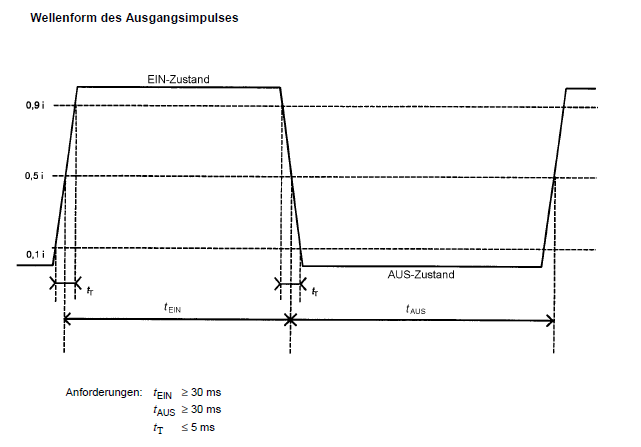
\includegraphics[width=0.70\textwidth]{Bilder/S0_Impulsform.png}
		\quelle{[asd]}
\end{figure}

F�r die Zust�nde sind die folgenden Impulsl�ngen definiert:
\begin{description}
	\item[] Ein Impuls, im \underline{High- bzw. Ein- Zustand}, ist mit t$_{EIN}\geq$ 30 ms, also gr��er gleich 30 ms definiert und der
	\item[] \underline{Aus- bzw- Low-Zustand}, f�r die Zeit zwischen zwei aufeinanderfolgenden Impulsen, mit t$_{AUS}$ $\geq$ 30 ms, also gr��er gleich 30 ms
\end{description}
Dabei muss die �bergangszeit der Anstiegs- oder Abfallzeit zwischen den einzelnen Zust�nden, also der Zustandswechsel 5 ms sein.


\section{Datendarstellung}
\label{sec:Datendarstellung}
Bei der Datenhaltung, also der Datenspeicherung, gibt es verschiedene M�glichkeiten:
die Daten k�nnen beispielsweise als CSV, also als Comma Separated Values,
abgespeichert werden. Es gibt jedoch auch die M�glichkeiten die Daten in
JSON oder aber auch in SQL abzulegen. Die Daten in SQL abzuspeichern lohnt sich
erst, wenn die Daten auch lokal auf dem Raspberry Pi weiterverarbeitet werden sollen.
Dabei muss auch bedacht werden, dass ein SQL-Server ben�tigt wird. Dies
w�rde dazu f�hren, dass durch den SQL-Server mehr Ressourcen verwenden w�rden.
Das hei�t ein SQL-Server w�rde nicht nur Speicher auf der SD-Karte einnehmen,
sondern auch, wenn der Server l�uft, den Arbeitsspeicher und die CPU beanspruchen.

Beim JSON ist bei der Programmierung des Quellcodes, die auf dem Raspberry Pi
l�uft, nur ein Libary n�tig, der die Daten in eine. JSON-Datei schreibt. JSON wird
meist im Web Bereich eingesetzt.


\subsection{Comma Separated Values (CSV)}
\label{sec:CommaSeparatedValuesCSV}
emeinen
Standard oder bestimmte Spezifikation, sondern es kann in unterschiedlichen
Spezifikationen eingesetzt werden. Das CSV-Format kann dann eingesetzt,
wenn die abgespeicherten Daten unabh�ngig von der Technologie eingesetzt werden
sollen. Also wenn die Daten beispielsweise in einem Tabellenprogramm dargestellt
und in einem Quellcode bearbeitet werden sollen \cite[vgl.]{RFC4180}.

Die Daten k�nnen entweder durch einfache Kommata voneinander getrennt in der
.csv Datei abgelegt werden, die Werte an sich k�nnen zus�tzlich in Anf�hrungsstriche
bzw -zeichen gesetzt werden. Genauso k�nnten die einzelnen Daten mit Semikolon
voneinander getrennt abgespeichert werden \cite[vgl.]{RFC4180}. Zu beachten ist
jedoch, dass bei Kommazahlen im deutschen ein Komma benutzt wird und im englischsprachigen
Raum ein Punkt. Dies k�nnte evtl. zu Problemen beim Lesen bzw.
Parsen der Datei im Quellcode f�hren.


\subsection{JavaScript Object Notation (JSON)}
\label{sec:JavaScriptObjectNotationJSON}
JavaScript Object Notation, kurz JSON, ist ein Datenaustauschformat. Dabei handelt
es sich um ein von Programmiersprachen unabh�ngiges Textformat. Daten k�nnen
also programmiersprachenunabh�ngig ausgetauscht werden. JSON folgt jedoch
der JavaScript Notation. Dabei handelt es sich bei JSON um eine Untermenge der
Skriptsprache JavaScript \cite[vgl.]{ecma2013}.

Das Datenaustauschformat basiert dabei auf zwei Strukturen \cite[vgl.]{ecma2013}:
\begin{description}
	\item \textbf{Name-Wert-Paare}\\	
	Dabei ist jedem Namen bzw. Bezeichnung mindestens ein Wert zugewiesen.
	
	\item \textbf{Geordnete Liste von Werten}\\
Neben den beiden Strukturen gibt es in JSON, wie auch in Programmiersprachen, Typen. Die Typen beziehen sich auf die Werte. Die folgende Auflistung mit entsprechenden Zeichen
[vgl ecma2013]:

	\item \textbf{Objekte}\\
\textit{Objekte} beinhaltet eine ungeordnete Menge an Name-Werte-Paare. Es beginnt mit einer �ffnenden geschweiften Klammer "`{"` und einer schlie�enden geschweiften Klammer "`}"'. Die Name-Werte-Paare sind mit einem Doppelpunkt getrennt [vgl. ecma2013]:\\
\item \textit{Name:Wert}\\
Jedes Paar ist wiederum zueinander mit Kommata (,) voneinander getrennt [vgl. ecma2013].

	\item \textbf{Arrays}\\
Ein Array beinhaltet eine geordnete Liste von Werten, die einem Namen zugewiesen werden. Arrays beginnen mit einer [ (�ffnenden eckigen Klammer) und enden mit einer ] (schlie�enden eckigen Klammer). Die Werte an sich sind mit , (Komma) zu einander getrennt [vgl ecma2013].

\item \textbf{Werte}\\
Werte werden durch Objekte, Arrays, Zeichenketten (Strings), Zahlen, den Wahrheitswerten \textsl{true} und false oder Null gebildet [vgl ecma2013].
\item \textbf{Zeichenketten}\\
Strings, also Zeichenketten, sind Unicode Zeichen [vgl ecma2013].

\item \textbf{Nummern}\\
Bei den Zahlen in JSON handelt es sich um Dezimalzahlen. Den Zahlen kann ein -
(Minus) vorangestellt werden. Gefolgt von entweder einem 0 (Null) oder einer beliebigen Zahl von 1 bis 9 in beliebiger Weiderholung. Gleitkommerzahlen werden mit einem Punkt getrennt [vgl ecma2013]. \cite{ecma2013}
\end{description}
Im Folgenden ist ein beispielhafter Aufbau einer JSON-Datei dargestellt:

\newpage
\begin{lstlisting}[language=json, caption={Beispielhafter Aufbau einer JSON-Datei}]
{
	"`books"': [
		"`book"': {
			"`language"':"'Java"',
			"`edition"':"'second"',
			"`price"': 10,
			"`author"': ["`Hans"', "`Peter"', "`M�ller"']
		},

		"`book"': {
			"`language"':"'C++"',
			"`lastName"':"'fifth"'
			"`price"': 11.12,
			"`author"': ["`Stroustroup"']
		},

		"`book"': {
			"`language"':"'C"',
			"`lastName"':"'third"'
			"`price"': 8,
			"`author"': ["`Georg"', "`Petrus"']
		}
	]
}
\end{lstlisting}
\begin{center}
\quelle{\cite[vgl.][]{asd}}
\end{center}



\chapter{Anforderungsdefinition}
\label{sec:KapAnforderungsdefinition}
F�r das Monitoring von Energieverbrauchswerten soll eine Softwarel�sung entwickelt werden. Es soll �ber die S0-Schnittstellen von Z�hlern Energieverbrauchswerte erfassen, anschlie�end verarbeiten und lokal abspeichern.

Die abgespeicherten Verbrauchswerte sollen an einen Server gesendet werden.

Die Visualisierung der Verbrauchswerte erfolgt grafisch �ber eine Weboberfl�che. Dabei werden 
die Energieverbrauchswerte entweder f�r einen bestimmten, vom Be-nutzer ausgew�hlten, 
Zeitraum abgefragt. Oder die aktuellen Verbrauchswerte werden fortlaufend von der
Messeinheit, also vom Aufsatz SD0 und dem Raspberry Pi abgefragt und auf dem Raspberry Pi 
dargestellt.

Die Verbrauchswerte werden �ber die S0-Schnittstellen des Aufsatzes SD0 gemessen. Die 
gemessenen Daten werden anschlie�end vom Aufsatz �ber die serielle Schnittstelle, also dem 
UART, des Raspberry Pi an diesen �bertragen. Auf dem Raspberry Pi werden die S0-Impulse 
verarbeitet und anschlie�end mit dem jeweiligen Zeitstempel des Zeitpunktes der Messung 
versehen und abgespeichert.

Die abgespeicherten Verbrauchswerte werden anschlie�end an einen Server weitergeleitet, wo 
die Verbrauchswerte f�r einen, vom Benutzer bestimmten, Zeitraum grafisch dargestellt werden. 
Der Server kann sich physisch an einem anderen Ort als der Raspberry Pi befinden. Dabei 
erfolgt die Kommunikation �ber die Ethernet Schnittstelle. Alternativ kann die Webdarstellung 
auf dem Raspberry erfolgen. F�r die fortlaufende grafische Darstellung des Energieverbrauchs 
muss sich die Webdarstellung auf dem Raspberry Pi befinden.

\section{Muss-Kriterium}
\label{sec:MussKriterium}

%Counter
\newcounter{MussKriterien}
\setcounter{MussKriterien}{0}
\newcommand{\MussKriterien}[1]{%
  \stepcounter{MussKriterien}%
  #10\theMussKriterien0
}


\textbf{\MussKriterien{M-ERF}} Erfassen der S0-Impulse am Z�hler\\
Durch S0-Impulse soll der Verbrauch am Stromz�hler erfasst werden.
\\

\addtocounter{MussKriterien}{-1}
\textbf{\MussKriterien{M-ERF}-10} Anzahl der verschiedenen, gemessenen Stromz�hlern\\
Mit dem Aufbau muss m�glich sein, an bis zu vier verschiedenen Stromz�hler Stromz�hlern mit S0-Schnittstellen die S0-Impulse erfasst zu k�nnen.\\7
\\

\textbf{\MussKriterien{M-ERF}} �bergabe der erfassten S0-Impusle an den Raspberry Pi\\
Die erfassten S0-Impulse werden nach dem Messvorgang dem Raspberry Pi �ber die GPIO-Schnittstelle �bergeben.\\

\textbf{\MussKriterien{M-VERA}}Umrechnung der �bergebenen S0-Impusle\\
Die gemessenen S0-Impusle, die an den Raspberry Pi �bergeben wurden, m�ssen auf dem Raspberry Pi in Energieverbrauchswerte (Watt pro Stunde) umgerechnet werden.
\\

\textbf{\MussKriterien{M-VERA}}Abspeichern von umgerechneten Energieverbrauchswerten.\\
Die von S0-Impuslen nach Energieverbrauchswerte umgerechneten Werte m�ssen auf dem Raspberry Pi abgespeichert werden.
\\

\textbf{\MussKriterien{M-SEN}} Senden der abgespeicherten Energieverbrauchsdaten.\\
Alle abgespeicherten Dateien sollen an einen Server versendet werden k�nnen.
\\

\textbf{\MussKriterien{M-SEN}-10} Zeiten f�r das Senden der abgespeicherten Energieverbrauchsdaten\\
Die abgespeicherten Dateien sollen zu bestimmten Uhrzeiten an einen Server versendet werden k�nnen.
\\

\textbf{\MussKriterien{M-SEN}-11}Zeiten f�r das Senden der abgespeicherten Energieverbrauchsdaten\\
Die abgespeicherten Dateien sollen permanent an einen Server versendet werden k�nnen.
\\

\textbf{\MussKriterien{M-BEA}} Betriebsart der Software\\
Die Software muss als Dienstprogramm laufen.
\\

\textbf{\MussKriterien{M-BEA}} Dauerhafter Betrieb der Software\\
Die Software muss dauerhaft auf dem Raspberry Pi laufen.
\\

\textbf{\MussKriterien{M-BEA}} Starten der Software\\
Die Software muss mit dem Systemstart der Raspberry Pi bzw. dessen Betriebssys-tems gestartet werden.
\\

\textbf{\MussKriterien{M-BEA}} Beenden der Software\\
Die Software muss vom Benutzer durch Angabe der Prozessnummer der Software beendet werden k�nnen.
\\

\textbf{\MussKriterien{M-BEA}} Neustart der Software\\
Die Software muss vom Benutzer neugestartet werden k�nnen.
\\

\textbf{\MussKriterien{M-KONF}} Einlesen einer Konfigurationsdatei\\
Die Software muss w�hrend der Laufzeit eine Konfigurationsdatei einlesen k�nnen.
\\

\textbf{\MussKriterien{M- KONF}} Einlesen der Impulskonstante einer Konfigurationsdatei\\
Die Software muss w�hrend der Laufzeit der Impulskonstante von bis zu vier unter-schiedlichen Stromz�hlern aus einer Konfigurationsdatei einlesen k�nnen.
\\

\textbf{\MussKriterien{M- KONF}} Einlesen der Empf�ngeradresse aus einer Konfigurationsdatei\\
Die Software muss w�hrend der Laufzeit die IP-Adresse, an die die gespeicherten Energieverbrauchswerte gesendet werden sollen, aus einer Konfigurationsdatei ein-lesen k�nnen.
\\

\textbf{\MussKriterien{M- KONF}-10} Einlesen der Empf�ngeradresse aus einer Konfigurationsdatei\\
Wird f�r die IP-Adresse, an denen die Daten gesendet werden sollen als Localhost oder 127.0.01 angegeben, verbleiben die Daten auf dem Raspberry Pi. Bei der Ad-resse handelt es sich um den Raspberry Pi selbst [vgl. loc].
\\

\textbf{\MussKriterien{M-KONF}}: Einlesen einer Konfigurationsdatei
Die Software muss w�hrend der Laufzeit eine Konfigurationsdatei einlesen k�nnen.
\\

\textbf{\MussKriterien{M- KONF}}: Einlesen der Impulskonstante einer Konfigurationsdatei
Die Software muss w�hrend der Laufzeit der Impulskonstante von bis zu vier unter-schiedlichen Stromz�hlern aus einer Konfigurationsdatei einlesen k�nnen.
\\

\textbf{\MussKriterien{M- KONF}}: Einlesen der Empf�ngeradresse aus einer Konfigurationsdatei
Die Software muss w�hrend der Laufzeit die IP-Adresse, an die die gespeicherten Energieverbrauchswerte gesendet werden sollen, aus einer Konfigurationsdatei ein-lesen k�nnen.
\\

\textbf{\MussKriterien{M- KONF}-10}: Einlesen der Empf�ngeradresse aus einer Konfigurationsdatei
Wird f�r die IP-Adresse, an denen die Daten gesendet werden sollen als Localhost oder 127.0.01 angegeben, verbleiben die Daten auf dem Raspberry Pi. Bei der Ad-resse handelt es sich um den Raspberry Pi selbst [vgl. loc].
\\

\textbf{\MussKriterien{M-DAR}}: Darstellung der umgerechneten Energieverbrauchswerte
Dem Benutzer sollen die umgerechneten Energieverbrauchsdaten grafisch darge-stellt werden.
\\

\textbf{\MussKriterien{M-DAR}-10}: Darstellung der umgerechneten Energieverbrauchswerten
Die grafische Darstellung der umgerechneten Energieverbrauchsdaten muss auf Webbasis geschehen.
\\

\textbf{\MussKriterien{M-DAR}}: Grafische Darstellung der umgerechneten 
Energieverbrauchswerten
Die grafische Darstellung der umgerechneten Energieverbrauchsdaten muss auf ei-nem Koordinatensystem geschehen.
\\

\textbf{\MussKriterien{M-DAR}}: Auswahl der Z�hler f�r die Darstellung der Energieverbrauchswerte
Der Benutzer soll f�r die grafische Darstellung die einzelnen Z�hler ausw�hlen k�n-nen. Die Verbrauchswerte der ausgew�hlten Z�hler werden dann auf einem Koordi-natensystem dargestellt.
\\

\textbf{\MussKriterien{M-DAR}-10}: Auswahl mehrerer Z�hler f�r die Darstellung der
Energieverbrauchswerte
Der Benutzer soll f�r die grafische Darstellung mehrere Z�hler gleichzeitig ausw�h-len k�nnen. Die Verbrauchswerte der ausgew�hlten Z�hler werden dann gleichzeitig grafisch auf einem Koordinatensystem dargestellt.
\\

\textbf{\MussKriterien{M-DAR}-20}: Auswahl aller Z�hler f�r die Darstellung der Energieverbrauchswerte
Der Benutzer soll f�r die grafische Darstellung alle Z�hler ausw�hlen k�nnen. Die Verbrauchswerte aller Z�hler werden, auf einem Koordinatensystem dargestellt.
\\

\textbf{\MussKriterien{M-DAR}}: Auswahl des Zeitraumes f�r die Darstellung der 
Energieverbrauchswerte
Der Benutzer muss f�r die grafische Darstellung den Zeitraum ausw�hlen k�nnen, in dem die 
Verbrauchsdaten angezeigt werden sollen.
\\

\textbf{\MussKriterien{M-DAR}-10}: Auswahl des Startdatums f�r die Darstellung der
Energieverbrauchswerte
Der Benutzer muss f�r die grafische Darstellung das Startdatum f�r den Zeitraum
Ausw�hlen k�nnen, bei dem die Verbrauchswerte angezeigt werden sollen, die ab dem ausgew�hlten Startdatum abgespeichert wurden.
\\

\textbf{\MussKriterien{M-DAR}-20}: Auswahl des Enddatums f�r die Darstellung der
Energieverbrauchswerte
Der Benutzer muss f�r die grafische Darstellung das Enddatum f�r den Zeitraum
ausw�hlen k�nnen, bei dem die Verbrauchswerte angezeigt werden sollen, die bis
zum dem ausgew�hlten Enddatum abgespeichert wurden.
\\

\textbf{\MussKriterien{M-DAR}-30}: Keine Auswahl des Datums f�r die Darstellung der
Energieverbrauchswerte
Ein bestimmtes Datum kann nicht ausgew�hlt werden, wenn f�r dieses Datum keine Energieverbrauchsdaten abgespeichert wurden.

\section{Kann-Kriterien}
\label{sec:KannKriterien}

%Counter
\newcounter{KannKriterien}
\setcounter{KannKriterien}{0}
\newcommand{\KannKriterien}[1]{%
  \stepcounter{KannKriterien}%
  #10\theKannKriterien0
}
\textbf{\KannKriterien{K-DAR}}Darstellung der aktuellen Energieverbrauchswerte\\
Dem Benutzer kann die M�glichkeit gegeben werden, die Energieverbrauchswerte darstellen zu lassen, die aktuell verbraucht werden.
\\

\textbf{\KannKriterien{K-DAR}}Export der Verbrauchsdatendarstellung in Bilddatei\\
Dem Benutzer kann die M�glichkeit gegeben werden, die von diesem betrachtete grafische Darstellung der Energieverbrauchsdaten in eine Bilddatei zu exportieren.



\section{Technische Kriterien}
\label{sec:TechnischeKriterien}

%Counter
\newcounter{TechnischeKriterien}
\setcounter{TechnischeKriterien}{0}
\newcommand{\TechnischeKriterien}[1]{%
  \stepcounter{TechnischeKriterien}%
  #10\theTechnischeKriterien0
} 

\textbf{\KannKriterien{MT}}: Den Aufsatz SD0 benutzen
F�r die Messung der S0-Impulse muss der Aufsatz SD0 von Busware benutzt wer-den.
\\

\textbf{\KannKriterien{MT}}: Datenempfang vom Aufsatz SD0 
Die gemessenen S0-Impulse sollen vom Aufsatz SD0 von Busware �ber die serielle Schnittstelle empfangen werden.


\chapter{Entwurf}
\label{sec:KapEntwurf}
\section{Anwendungsf�lle der zu entwickelnden Software}
\label{sec:51Anwendungsf�lleDerZuEntwickelndenSoftware}



\chapter{Realisierung}
\label{sec:KapRealisierung}
In diesem Kapitel wird die Realisierung der prototypischen Entwicklung beschrieben.

Um die Verbrauchswerte zu messen gibt es schon ein Projekt, den Volksz�hler. Da-bei handelt es sich um ein Open Source Projekt [vgl. vza]. Mit dem Volksz�hler k�n-nen Energieverbrauchswerte gemessen und auf dessen Darstellung Verbrauchswer-te von Wasser, Strom Gas usw. angezeigt werden [vgl. Zoe], mit dem die Nutzer die eigenen Verbrauchdaten wie Strom, Temperatur, Wasser am Z�hler messen k�nnen. Die gemessenen Verbrauchsdaten werden dann �ber die Schnittstellen an das Messger�t �bertragen, dort gespeichert und auf einer Website ausgewertet. Ein ge-eignetes Messger�t muss vorhanden sein. In dieser Arbeit handelt es sich dabei um den SD0 von Busware, zusammen mit dem Raspberry Pi. Die Messung findet dabei am Z�hler �ber die S0-Schnittstelle statt. Die �bertragung findet �ber Kupferkabel statt. Die Speicherung und Auswertung finden dann durch die Software statt. Bei der Software handelt es sich um den Volksz�hler. Mit dem Volksz�hler k�nnen auch Verbrauchsdaten �ber S0-Schnittstellen gemessen werden [vgl. vzg]. Dazu gibt es zwei Softwares, um S0-Impulse zu messen. Dabei handelt es sich um s0vz [vgl. s0vz] und s0enow. Aus dem Quellcode bzw. der Datei s0enow.cpp, in der sich auch die Main-Funktion befindet, geht hervor, dass sich beim Projekt s0enow um einen nach GNU General Public Licence der Version 3 Lizenzierte Software handelt. Das bedeutet, dass der Quellcode verwendet bzw. Modifiziert werden darf. Dabei muss aber die Software, die Teile der Software, die nach GNU General Public Licence der Version 3 lizenziert wurde, verwendet auch als solche lizenziert werden [vgl. s0ec Codezeilen 23 bis 38] \cite[vgl.][S. 455]{s0ec}.

In dieser Arbeit werden einige Funktionen, die im Softwareprojekt s0enow vorhanden sind, verwendet. Dadurch m�ssen diese nicht von neuem entwickelt werden. Neben der Bibliothek, die zum Einlesen der Konfigurationsdatei dient, werden �hnliche Da-ten eingelesen, wie im Projekt s0enow. Dies ist der Tatsache geschuldet, dass die Software die in dieser Arbeit entwickelt wird, eine �hnliche Aufgabe erf�llt, wie das Projekt s0enow. Dabei handelt es sich um die Funktion cfile(). Diese Datei befindet sich in den Codezeilen 204 bis 309 im s0enow Projekt [vgl. s0ec].
In der Software, die in dieser Arbeit entwickelt wird, werden neben dem Datafolder, die Messstellenname, die Mittelwertszeit auch die Impulskonstanten ausgelesen.

Zus�tzlich gibt es �berschneidungen mit den Projekten s0enow und s0vz. Wie in diesen Projekten wird die Software, die auf dem Raspberry Pi laufen soll, als Dienst-programm bzw. Deamon entwickelt So genannte Deamons laufen unter Linux im Hintergrund und starten, wenn das Betriebssystem hochgefahren wird [vgl. Wol2006 dpz und Wol2006 af]. Diese Funktionen befinden sich in den Codezeilen 111 bis 202, im Projekt s0enow [vgl. s0ec]. Bei den Funktionen handelt es sich um die drei fol-genden Funktionen,



\chapter{Inbetriebnahme}
\label{sec:KapInbetriebnahme}
\section{Zielbeschreibung}
\label{sec:Zielbeschreibung}


\chapter{Test}
\label{sec:KapTest}
\input{8_Kap/8_Test}


\chapter{Zusammenfassung und Ausblick}
\label{sec:KapZusammenfassungUndAusblick}
In dieser Abschlussarbeit wurde eine, aus zwei Bereichen bestehende, Softwarel�sung
entwickelt, die den eigenen Energieverbrauch visualisiert und dadurch die M�glichkeit
aufgreift den eigenen Energieverbrauch zu analysieren. Die auf der Grundlage eines
Linux-Betriebssystems entwickelte Software, welche auf einem Raspberry Pi l�uft,
wertet die empfangenen S0-Impulse in Energieverbrauchswerte um. Auf der Grundlage,
von diesen als Linuxtreiber (auch Deamon bezeichnet) entwickelten Software
ausgewerteten Verbrauchswerten, findet die Visualisierung, der ausgewerteten
Energieverbrauchswerte statt. Die Visualisierungseinheit, also die Webseite befindet
sich dann auf einem Webserver, der entweder auf einem Raspberry Pi oder einem vom
Raspberry Pi physisch unabh�ngigen Server l�uft. Die entwickelte Visualisierungseinheit
bietet den Vorteil, dass nicht nur der bisherige Gesamtverbrauch, vom Z�hler als
Zahl abgelesen werden kann, sondern die Verbrauchswerte f�r einen bestimmten
Zeitraum grafisch darzustellen werden. Zudem ist es durch die Auswahl der einzelnen
Kan�len, die der Anzahl der S0-Anschl�ssen der Erweiterung SD0 entsprechen, m�glich
die Verbrauchswerte verschiedener Z�hler, gleichzeitig zu analysieren und miteinander
zu vergleichen. Es wurde eine Anforderungsanalyse durchgef�hrt, die die Anforderungen
an die entwickelte Softwarel�sungen definieren soll. Mit deren Hilfe wurden dann
im anschlie�enden Kapitel die L�sungen entworfen. Ausgehend vom Entwurf, der die
Grundlage bzw. den Ausgangspunkt der realisierten L�sungen bildet, wurde die L�sung
realisiert. Es wurde auch ein Parser zum Einlesen von Konfigurationsdateien verwendet.
Dadurch kann die Software w�hrend der Laufzeit an verschiedene Z�hler angepasst
werden. Die Software, die auf dem Raspberry Pi l�uft, wurde modular aufgebaut.
Dadurch ist sp�ter eine einfache Erweiterung der schon entwickelten Software m�glich.

Der Vorteil bei der in dieser Abschlussarbeit eingesetzten S0-Schnittstelle ist,
dass die Schnittstelle nicht nur f�r den Energieverbrauch, sondern auch f�r andere
Verbrauchswerte wie W�rme, Wasser und Gas verwendet werden kann. Die entwickelte
Software kann also in Verbindung mit den S0-Schnittstellen vielseitig verwendet
werden.

Eine M�glichkeit den Prototyp zu erweitern w�re, weitere Darstellungsformen und 
-varianten hinzuzuf�gen. Das w�re beispielsweise die Darstellung der Verbrauchsdaten
in einer App, also auf einem Smartphone oder Tablet. Es w�re auch m�glich, weitere
Daten, wie Tarifinformationen und bisherige Kosten f�r den Energie-verbrauch,
darzustellen. Es w�re auch m�glich, die aktuellen Energieverbrauchswerte mit den
Verbrauchswerten des selben Zeitraums vergangener Jahre zu vergleichen.

\appendix							% Beginn des Anhangs
\pagenumbering{Roman}
\newpage
%\addcontentsline{toc}{chapter}{Tabellenverzeichnis}
\listoftables				% Tabellenverzeichnis

\newpage
%\addcontentsline{toc}{chapter}{Abbildungsverzeichnis}
\listoffigures				% Abbildungsverzeichnis

\newpage
%\addcontentsline{toc}{chapter}{Quellcodeverzeichnis}
\lstlistoflistings				% Quellcodeverzeichnis

\nocite{*}
\printbibheading                    % print heading for all bibliographies
\newpage
\printbibliography[nottype = online, title = Literaturverzeichnis]
\printbibliography[
		type = online,                    % Put only references of the type "online" here.
		title = {Online-Quellen},
		heading = subbibliography
]

\pagenumbering{gobble}
\ofoot{}
% Beginn des Anhangs

\renewcommand{\thesection}{\Alph{section}}
\appendix
\addchap{Anhang}
\section{Schaltplan des Raspberry Pi Model B}
\label{sec:SchaltplanDesRaspberryPiModelB}
\newpage

\section{Schaltplan des SD0}
\label{sec:SchaltplanDesSD0}
\newpage
	
\section{Hilfsfunktionen zum zeichnen der Energieverbrauchsdaten}
\label{sec:HilfsfunktionenZumZeichnenDerEnergieverbrauchsdaten}
\newpage

\section{Inhalt und Struktur der Beiliegenden CD}
\label{sec:InhaltUndStrukturDerBeiliegendenCD}

%\backmatter					% Nachspann 

%% Bibliographie unter Verwendung von dinnat %%%%%%%%%%%%%%%%%%%%%%%%%%
%\setbibpreamble{Pr�ambel}		% Text vor dem Verzeichnis
%\bibliographystyle{dinat}
%\bibliography{bibliographie}	% Sie ben�tigen einen *.bib-Datei
\end{document}